% Monografia para Projeto de Fim de Curso - Exemplo no LaTeX
%-----------------------------------------------------------


%---------------Inicialização de pacotes--------------------

\documentclass[12pt,a4paper,notitlepage,twoside]{book}
\usepackage{times}

\usepackage{graphicx}
\usepackage[utf8]{inputenc}
\usepackage[brazil]{babel}
\usepackage[T1]{fontenc}
\usepackage{amsmath}
\usepackage{amsthm,amsfonts}
\usepackage{color}
%\usepackage{hyperref}
\usepackage{abntex2abrev}


\usepackage[a4paper,top=30mm,bottom=30mm,inner=30mm,outer=25mm,headheight=7mm,headsep=6mm,footskip=7mm]{geometry}
%\usepackage{epsfig}
%\usepackage{latexsym}
%\usepackage{float}
%\usepackage{quotes}
%\pagestyle {plain}

\makeindex

\def\baselinestretch{1.0}

%---------------Início do documento-------------------------

\begin{document}

\begin{titlepage}
\begin{center}
{\large Universidade Federal de Minas Gerais\\
Escola de Engenharia \\
Curso de Graduação em Engenharia de Controle e Automação\\}

\vspace{6cm}
{\bf\Large Primeira Linha do Título\vspace{0.2cm}

Segunda Linha do Título, se Houver}
\vspace{4cm}

%\hspace{0.3\textwidth} \parbox{0.65\textwidth}
{\large André Sales Barbosa}
\vspace{2cm}  
   
\vspace{2cm}          
%\hspace{0.3\textwidth} 
{\large Orientador: Prof. Antônio de Pádua Braga, Dr.}\\


\vfill
%\hspace{0.3\textwidth} 
{\large Belo Horizonte, Dezembro de 2017 }
\end{center}

\end{titlepage}

\newpage
\clearpage
\thispagestyle{empty}


\begin{titlepage}

\centering
\textbf{Monografia}\\
\vspace{2cm}
\centering
\textbf{Título da Monografia}\\
\vspace{5cm} 

\parbox{1.0\textwidth} 
{\large 
Monografia submetida à banca examinadora
designada pelo Colegiado Didático do Curso de
Graduação em Engenharia de Controle e
Automação da Universidade Federal de Minas
Gerais, como parte dos requisitos para aprovação na
disciplina Projeto Final de Curso II.}

\vspace{7cm} 
\centering
Belo Horizonte, Dezembro de 2017

\end{titlepage}

\clearpage
\thispagestyle{empty}
\cleardoublepage

\pagenumbering{roman}
\section{Descrição do problema e solução proposta}

Esse trabalho de projeto de final de curso se dedica à implementação do algoritmo
 de reconhecimento de padrões para classificar movimentos.
Para isso faz-se o uso de uma placa de desenvolvimento do  microcontrolador ESP32 e um sensor 
acelerômetro MPU6050. O protótipo desenvolvido deverá reconhecer qual movimento foi aplicado
 ao objeto e exercer uma atuação a partir disso.
 A inspiração para o projeto veio do conceito de inteligência distribuída. Nessa abordagem o
 algoritmo de inteligência artificial é implementado nos dispositivos de borda ("edge"), evitando
 a transferência de dados para um processamento central.

\addcontentsline{toc}{chapter}{Agradecimentos}

\begin{center}
\huge{{\bf Agradecimentos}}
\vspace{4cm}
\end{center}

Aqui vai o texto dos agradecimentos.
 
\clearpage
\thispagestyle{empty}
\cleardoublepage
\tableofcontents
%\markboth{Conteúdo}{Conteúdo}

\clearpage
%\thispagestyle{empty}
%\cleardoublepage

% Normalmente, este arquivo só contém isto.
\listoffigures
\addcontentsline{toc}{chapter}{Lista de Figuras}
%\markboth{Lista de Figuras}{Lista de Figuras}

\clearpage
%\thispagestyle{empty}
%\cleardoublepage

% Normalmente, este arquivo só contém isto.
\listoftables
\addcontentsline{toc}{chapter}{Lista de Tabelas}
%\markboth{Lista de Tabelas}{Lista de Tabelas}

\clearpage
%\thispagestyle{empty}
%\cleardoublepage

% Normalmente, este arquivo só contém isto.

\pagenumbering{arabic}
\setcounter{page}{1}
\chapter{Introdução}
%\markboth{\thechapter ~~~ Introdução}{}
%\label{intro}

Se preferir, você pode apresentar este Capítulo antes da primeira Seção, destacando os principais pontos que são abordados. %\cite{Raffo2008}

\section{Motivação e Justificativa}
\markright{\thesection ~~~ Motivação}
%\label{motiva}


\section{Objetivos do Projeto}
\markright{\thesection ~~~ Objetivos}
%label{objetivos}

Tendo em vista o exposto acima, este projeto tem por objetivos:

\begin{itemize}
\item[a.] Item 1;
\item[b.] Item 2;
\item Etc.
\end{itemize}




\section{Local de Realização}
\markright{\thesection ~~~ A Empresa}
%\label{empresa}

Vale à pena descrever a empresa onde o PFC foi desenvolvido. Veja o exemplo abaixo.

O projeto de fim de curso foi desenvolvido na empresa ..., no Departamento de ..., responsável por toda a implementação do sistema de ...

A empresa realiza projetos de pesquisa e desenvolvimento, consultoria e treinamento nas áreas de ...

A ... foi criada em ...  

A empresa é divida em três departamentos: (o arquivo Introducao.tex mostra como criar a lista abaixo) 

\begin{itemize}
\item Departamento de ... 
\item Departamento de ...
\item Departamento de ...
\end{itemize}

Este projeto foi desenvolvido no Departamento de ..., que é o responsável por ...

Os demais Departamentos englobam as fun\c{c}\~oes de ...

Todos os departamentos trabalham em conjunto. O Departamento de ..., por exemplo, precisa manter um grande vínculo com o Departamento de ... Isso ocorre porque todas as especifica\c{c}\~oes de hardware e sistemas influenciam a forma de implementa\c{c}ão de servi\c{c}os, organiza\c{c}\~ao de tabelas e recursos disponíveis.




\section{Estrutura da Monografia}
\markright{\thesection ~~~ Organização do Trabalho}
%\label{organiza}

O trabalho está dividido em quatro capítulos. Este capítulo apresentou uma introdução ao projeto a ser descrito nesta monografia e a empresa onde o trabalho foi realizado. O Capítulo 2 descreve os princípios básicos de um sistema ... (sistema onde se insere o trabalho) e abrange todos os conceitos necessários para um melhor entendimento do projeto. O Capítulo 3 aborda a metodologia de desenvolvimento, seguida pela implementa\c{c}\~ao dos .... No Capítulo 4 tem-se a conclusão da  monografia e algumas sugest \~oes e dificuldades encontradas na realização do projeto.


\clearpage
\chapter[Descrição do Processo]{Descrição do Problema/Processo ou O Processo de Fazer Alguma Coisa}
\label{chap:descricaoproblema}
%Note que, como nome do capítulo é muito longo, fornecemos um nome abreviado uso no cabeçalho

Se desejar, uma visão geral do capítulo pode ser colocada antes da primeira seção. Este é o capítulo de descrição do processo e formulação do problema. Tendo em vista que se trata de uma monografia de engenharia de controle e automação, em muitos casos será fundamental a apresentação dos sensores e atuadores do processo.


\section{Processo de Fazer Alguma Coisa}
\label{sec:hist}

Cada seção inicia pela descrição do seu conteúdo e pode terminar com um parágrafo de conexão com a seção seguinte. 

Antes de formular o problema, \textbf{não se esqueça de fazer todas as definições necessárias}. Também devem-se detalhar os aspectos complementares da abordagem: se estamos estudando um aspeto particular do problema, se a resposta encontrada é universal ou dependente de simplificações e hipóteses prévias.


\section{Instrumentação do Processo}
\label{sec:instrumentação}

Descreva a aparelhagem e o equipamento utilizados bem como a ligação entre os diversos componentes. Nesta seção e, ao longo de todo o texto, você deve dar detalhes suficientes para que qualquer pessoa consiga reproduzir seus experimentos.

Contudo, \textbf{não disperse o leitor com detalhes irrelevantes} ou aspectos
demasiado técnicos ou formais. Reserve tais detalhes para um
apêndice.

Como uma imagem vale mais que mil palavras, e como usar mil palavras prejudicaria a clareza do texto, ilustramos o processo com a Figura \ref{fig:processo}. Lembrar que toda figura deve ser comentada no texto, você nunca deve colocar figuras que fiquem ``soltas'' no texto.  

\begin{figure}[thpb]
  \centering
  \resizebox{120mm}{!}{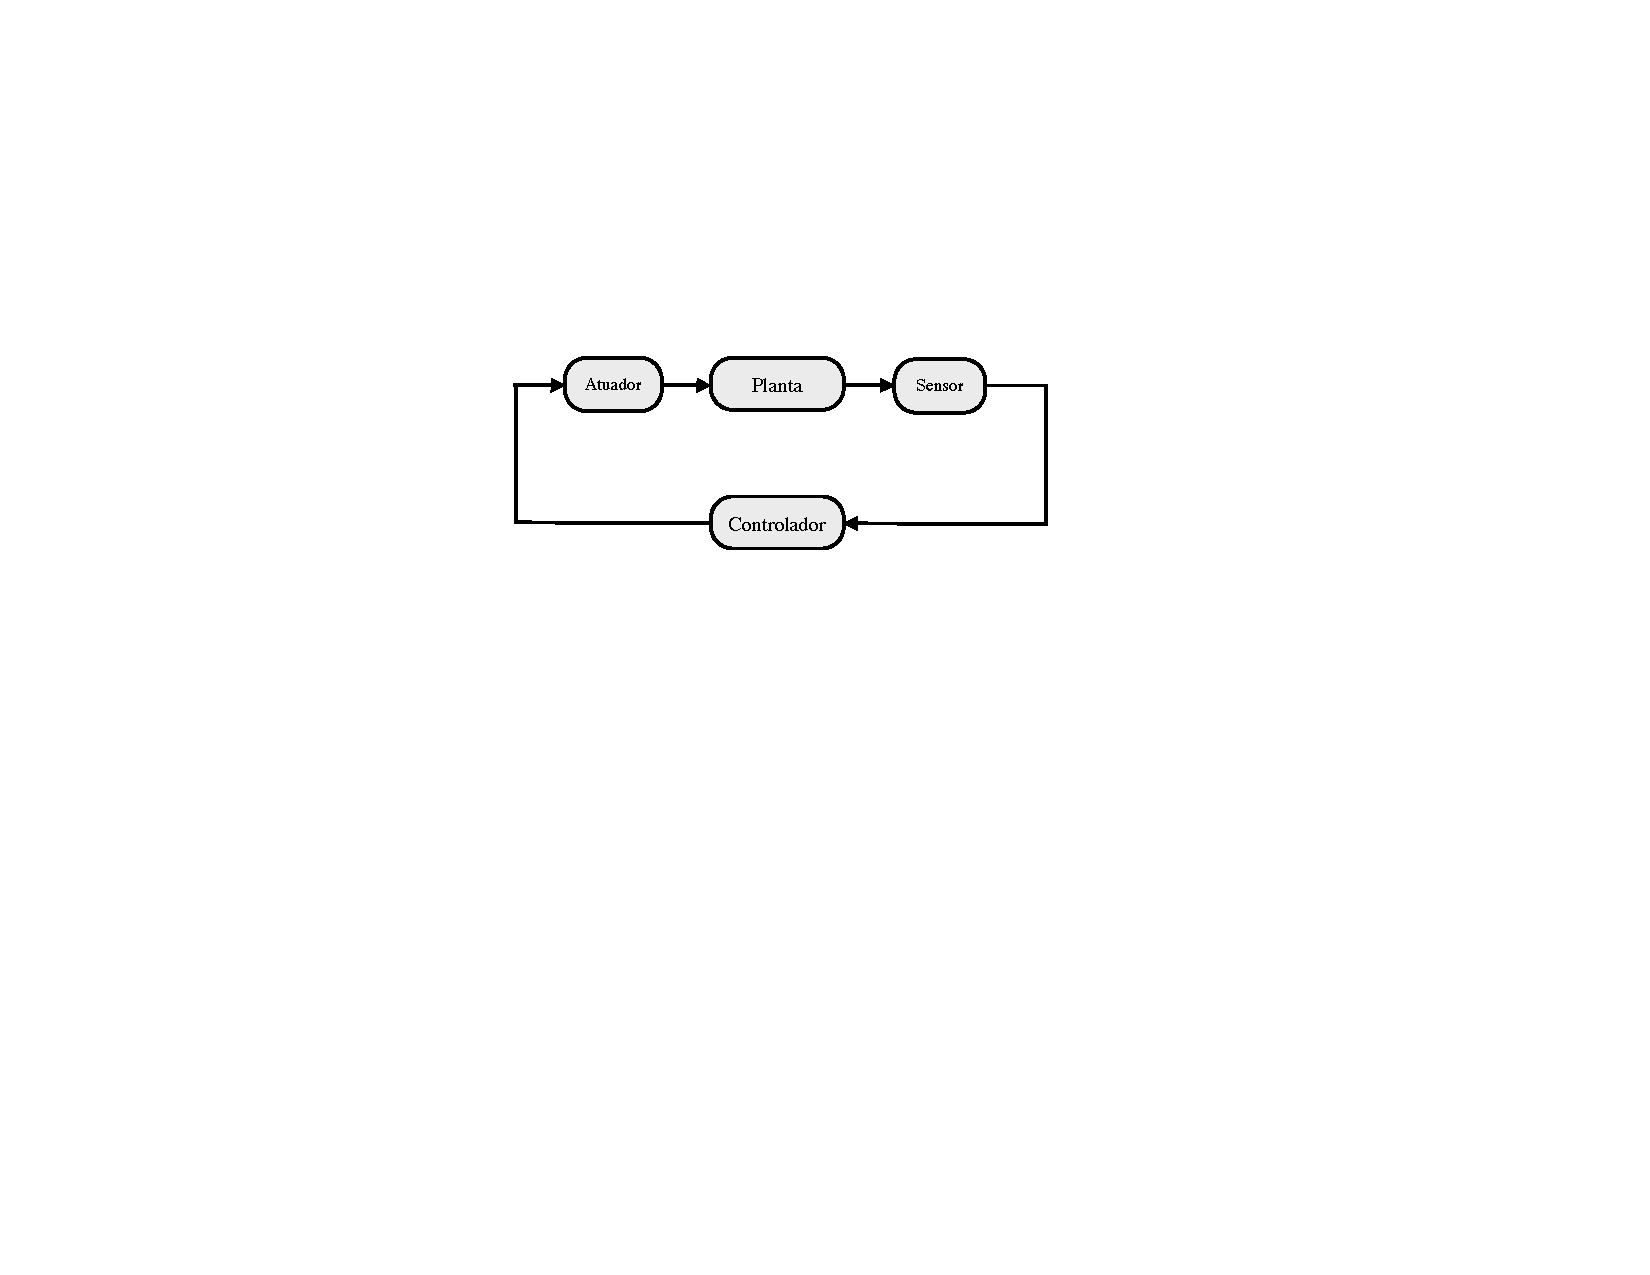
\includegraphics{DescricaoProcesso/Figuras/FiguraProcesso.pdf}}
  \caption{Aqui escrevemos \textbf{toda} informação pertinente à figura. Ou seja, este texto deve ser uma descrição auto-contida da figura, não sendo necessário recorrer ao corpo de texto para saber detalhes sobre a mesma. \emph{Fonte:} Citar fonte se figura 	não for elaborada pelo autor e \textbf{pedir permissão para usar!}}
  \label{fig:processo}
\end{figure}


\section{Situação Atual/Estado da Arte/Revisão da Literatura}
\label{sec:revisão}

Este é o espaço para uma revisão detalhada do enquadramento do problema. Isso inclui descrever a situação atual do processo, aquilo que foi feito até então dentro da empresa/laboratório, e aquilo que se pode chamar de ``Estado da Arte'', ou seja, uma apresentação do conhecimento preexistente
sobre o tema do projeto.

A elaboração desta seção tipicamente demanda uma boa revisão da literatura. Deve haver, quando aplicável uma análise das soluções potencialmente concorrentes, elencando vantagens e desvantagens.

\subsection{Como Elaborar uma Revisão da Literatura}

Ao selecionar referências, devem-se preferir referências de veículos confiáveis, que tenham por exemplo processo de revisão por pares. Portanto, dá-se preferência a artigos em periódicos e livros, em seguida teses e dissertações, artigos em anais de congresso e por fim relatórios. Evitar citar páginas da internet por oferecem menor garantia da informação nelas contida. 

Pesquise sua bibliografia em bases confiáveis como o \textsf{Web of Science}, \textsf{Scopus}, ou o \textsf{Google Scholar}. \textbf{Não use uma ferramenta de busca comum!} (elas não foram feitas pensando no \emph{ranking} de textos científicos) Use o número de citações de uma dada referência como um indicador de sua qualidade. Explore os artigos que citam a referência estudada bem como os artigos que ela cita.

Prefira as referências mais recentes quando se tratar de um assunto na fronteira do conhecimento ou de tecnologia de ponta. Quando se tratar de um assunto já consolidado, prefira citar livros ou artigos com muitas citações. 

Evite citar informações de segunda-mão e procure na medida do possível rastrear a fonte original. Contudo, em situações em que a fonte original é de acesso mais difícil, seja por ter tido publicação limitada como no caso de relatórios ou por não ser em língua inglesa ou portuguesa, é preferível a citação de segunda-mão em um veículo mais acessível.

Para gerenciar suas referências, use uma ferramenta de software como o \textsf{Mendeley}, que permite gerar arquivos .bib para uso em {\LaTeX} ou simplesmente gerar a lista de referências para uso direto em editores de texto. Em \LaTeX, mais especificamente Bib\TeX, a lista de referências é criada a partir de um arquivo .bib, que é uma espécie de banco de informações bibliográficas em que cada entrada é uma referência associada a uma chave para citação. A lista criada incluirá apenas as referências citadas ao longo do texto, mesmo que haja mais referências no arquivo .bib. As informações bibliográficas no formato Bib\TeX também podem ser obtidas para cada referência em ferramentas como o \textsf{Google Scholar} e então coladas no arquivo .bib.

Na Seção \ref{sec:comocitar} discutiremos como e quando as citações devem ser usadas.

\section{Resumo do Capítulo}

Tente não terminar de forma abrupta. Se for escrever algo aqui, não seja genérico!


\clearpage

\chapter{Metodologia}
\label{chap:metodologia}

Este capítulo deve descrever os métodos utilizados no projeto. As teorias e ferramentas utilizadas, assim como as ações executadas, devem ser escritas de forma clara e precisa, sem deixar espaço para ambiguidades. Tenha em mente que \textbf{o objetivo aqui é dar credibilidade ao seu trabalho e permitir que ele possa ser reproduzido por quem tenha interesse (algumas vezes por você mesmo!)}. 

É natural que este capítulo contenha uma revisão bibliográfica mais detalhada das técnicas utilizadas. O ideal é que o capítulo seja auto-contido, de modo que o leitor não necessite recorrer às referências para entender seu trabalho ou reproduzi-lo.

Ao apresentar os métodos, será importante justificar devidamente as opções tomadas e discutir as alternativas disponíveis e os critérios que o levaram à escolha do método.

No restante do capítulo, apresentamos um pequeno manual de escrita técnica.

\section{Técnica 1 - Organização do texto}
\label{sec:metodo1}

Procure \textbf{definir a estrutura} de seu texto \textbf{antes de começar a escrever}. Isso evitará que as ideias apareçam foram de ordem. A falta de organização é uma das características mais comuns de textos difíceis de ler.

Nunca invoque conceitos ou objetos antes de defini-los. Procure fornecer o máximo de informação \emph{a priori} possível. Evite referências para frente no texto. 

Para evitar que o leitor se perca, antes de iniciar um trecho longo de texto que contenha ideias diversas, \textbf{adiante para o leitor o que será feito}, aonde se quer chegar. Ao fim do trecho, declare explicitamente que chegou à conclusão que desejava. Esta técnica vale especialmente para seções e capítulos do texto. 

\section{Técnica 2 - Estilo}
\label{sec:estilo}

O texto técnico deve ser preciso, claro, sem ambiguidades, objetivo e conciso. Mesmo com esse rigor, não deixe de prender a atenção do leitor. Lembre-se de que o início e o fim de cada parágrafo, de cada frase, são as partes mais importantes e onde você deve colocar maior ênfase.


\subsection{Precisão}

Use as palavras corretas! Não escreva redondo se é esférico. Não escreva igual se é aproximado. Não escreva sistema se é função de transferência. Não escreva grande, pequeno, máximo, mínimo, ótimo, se não há uma escala que defina tais conceitos.

Prefira usar números que deem uma noção de escala a usar adjetivos difíceis de precisar.

Seja específico e evite generalidades. Por exemplo, em vez de dizer ``O processo 1 é um processo de alto custo'', devemos ser mais precisos com relação à natureza do custo e dizer ``O processo 1 possui custo operacional elevado com relação a processos tradicionais tais como o processo 2''.

\subsection{Clareza}

Não deixe margem para dúvidas! Para reduzir a possibilidade de confusão na leitura do seu texto, \textbf{evite frases longas}. Nunca escreva frases com mais de $20$ palavras. Procure escrever na média $12$ palavras por frase. Evite palavras compridas ou que possam ser consideradas difíceis.

Não deixe ideias subentendidas! Não assuma que seu leitor pensa como você e vai saber do que você está falando. Explicite todos os passos de seu raciocínio lógico. Pular passos de raciocínio é uma das causas mais comuns de confusão na leitura. Não seja preguiçoso neste quesito.

Novamente, defina todos os conceitos antes de fazer uso deles.

Não deixe o sujeito verbal subentendido. Para evitar ambiguidades, tome cuidado ao usar pronomes como ``esse, este, isso, ele''. É preferível repetir um nome a deixar margem para dúvidas. Por exemplo, após a primeira frase deste parágrafo poderíamos dizer de forma não tão clara: ``Esta é uma causa de confusão na escrita.''; ou poderíamos dizer de forma mais clara: ``Essa falta de informação é uma causa de confusão na escrita.''

Não há problemas em haver repetições em textos técnicos. O mais importante é a clareza, a inexistência de ambiguidades, não a beleza. Se acha que uma determinada frase pode ser confusa ou se alguma ideia parece difícil de explicar, repita a mesma ideia em outras palavras ou, melhor ainda, dê um exemplo.

Por fim, domine o significado das palavras utilizadas para evitar ambiguidades. Se uma palavra pode ter mais de um significado em determinada frase, tente trocá-la por outra que não deixe dúvidas. Mais importante ainda, não use palavras sobre cuja definição você não tem certeza.

\subsection{Ojetividade}

O texto técnico deve ser direto ao ponto, sem rodeios, e livre de opiniões. Evite apartes, evite divagações e discussões irrelevantes com relação ao tema principal.

\textbf{Nunca use hipérboles}. Cuidado com termos como ``otimizar, muito grande, enorme, muito bom''.  Usar números sempre que possível para quantificar conceitos, sejam eles precisos ou apenas uma estimativa. Em especial deve-se tomar cuidado com as palavras ``muito'' e ``muitos''.

O tom deve ser impessoal, apresentando apenas fatos e não opiniões. Em português, a voz passiva é um instrumento comum para se obter um tom impessoal. Contudo, sempre que possível, tente usar a voz ativa ou a voz passiva sintética para deixar o texto mais fluido e claro.

Palavras abstratas deixam a escrita vaga. Prefira palavras concretas, fortes, isto é, palavras que tenham um único significado. Sempre que possível substitua múltiplas palavras por uma única. Por exemplo, na frase ``A máquina processou as amostras'' temos duas palavras genéricas: máquina e processar. A mesma ideia seria mais objetiva se expressa como ``A centrífuga girou as amostras''.

Controle seu tom. \textbf{Não use linguagem coloquial. Não use clichês}. Não use de arrogância: ``obviamente, como é sabido, é claro que''. 

\subsection{Concisão}

O texto técnico deve ser tão curto quanto possível, sem prejuízo de sua clareza e precisão. Não use palavras a mais, não inclua expressões irrelevantes ou supérfluas. Não escreva simplesmente para encher as páginas. Se um assunto não é relevante para a compreensão do seu trabalho, corte-o, mova-o para um apêndice ou aponte uma referência.

Evite redundâncias como ``opinião pessoal'' e ``garantia absoluta''.

\section{Vícios comuns}

\begin{itemize}
\item Estrangeirismos: ``\emph{performance}'', ``\emph{mutatis mutandis}''. Se necessário, coloque o termo estrangeiro em itálico e dê uma tradução entre parênteses.

\item Usar linguagem rebuscada. Lembre-se de que a linguagem técnica deve ser clara, precisa e objetiva.

\item Alternar o tempo verbal entre passado e presente. Seja consistente e escreva apenas no passado ou no presente.

\item Iniciar uma frase com verbo porque o sujeito está implícito na frase anterior. Deixe sempre o sujeito explícito.

\item Inserir referências no meio de uma frase. Isso quebra o fluxo da leitura. Coloque a citação no fim da frase.

\item \textbf{Usar siglas sem antes defini-las}. Sempre escreva a sigla por extenso \emph{na primeira vez} que ela aparece no texto. Por exemplo, ``este é um texto de Projeto Final de Curso (PFC)''. 

\item Escrever ``como sabemos'', ``como é sabido'', ``por razões óbvias'', ``é evidente que'', ``talvez seja verdade que''. Estes termos significam apenas que você não sabe explicar o que está afirmando.

\item Usar definições \emph{por exemplo}, isto é, apresentar a definição de um conceito ou termo por meio de um exemplo. Primeiro defina o conceito, depois exemplifique.

\end{itemize}

\section{Boas práticas}

\begin{itemize}
\item Sempre que introduzir novos termos e conceitos, destaque-os em itálico para que o leitor saiba que se trata de uma definição e para que ele ache a definição com facilidade quando for necessário rastreá-la no texto.
\item Releia o que escreve a cada parágrafo. Releia rapidamente cada seção para verificar o encadeamento de ideias.
\item Corte palavras sempre que possível.
\item Nunca assuma que o leitor entenderá o que você escrever. Esforce-se para fazê-lo entender.
\item Use um corretor ortográfico.
\item Peça que alguém leia seu texto.
\end{itemize}


\section{Uso de referências}
\label{sec:comocitar}

Uma afirmação incluída num texto técnico se enquadra em um de três casos: a) seu conteúdo é de conhecimento geral dentro da área do texto; b) seu conteúdo é original e resulta do trabalho do autor; c) seu conteúdo tem origem em outro trabalho (ainda que seja do mesmo autor, não é original).

Toda afirmação enquadrada na categoria c) deve ser acompanhada de uma citação. Para afirmações da categoria b), deixe claro que se trata de ideia original do autor. Isso evita que o leitor se confunda ao pensar que possa se tratar de a) ou c).

No caso a), pode ser um tanto mais sutil determinar o que deve ser de conhecimento geral. Procure evitar o excesso de citações. Se todo um parágrafo se baseia em ideias de uma certa referência, em geral basta que ela seja citada no seu início.

\textbf{Atenção:} Não copie frases das referências usadas. Reescreva as ideias com suas próprias palavras e não deixe de citar a fonte. Se for necessário manter as palavras do original, cite a frase entre aspas e em itálico.

\section{Honestidade e Plágio}

Seja honesto ao escrever. \textbf{Não ``maqueie'' seus resultados}. Não apresente apenas as melhores amostras dos seus resultados para dar a impressão de que foi bem sucedido. Não escreva aquilo que não entende. Não escreva de forma vaga para mascarar o fato de que não entende algo.

Dê crédito a quem o merece. Inclua referências sempre que usar o trabalho de outros. Seja sempre claro para não dar a impressão de que fez algo feito por outrem. \textbf{Não assuma crédito pelo trabalho dos outros}. Isso pode ter implicações legais e acadêmicas.

\section{Cuidado com a gramática}

\begin{itemize}

\item Erros gramaticais deixam uma \textbf{impressão ruim} e podem alterar a disposição do leitor para com o texto.  

\item Use a vírgula corretamente. Seu uso incorreto confunde o leitor. Nunca use a vírgula porque acha que a frase precisa de uma pausa. Não separe sujeito e verbo. Quando há inversão da ordem natural em uma frase, \emph{toda} a parte movida deve estar entre vírgulas.

\item Cuidado com a concordância da voz passiva sintética. Lembre-se de que o correto é ``Vendem-se ovos'' e não ``Vende-se ovos''.

\item Use a crase corretamente. Faça sempre o exercício de substituir o nome que sucede o ``à'' por um nome no masculino. Se o correto for usar ``ao'' com o nome masculino, então deve haver crase. Nunca use crase antes de nomes no masculino!

\item Escreva ``em que'' em vez de ``onde'' quando não houver indicação de lugar.

\item Não se escreve ``o fato \textbf{dela} ser'' ou ``a razão \textbf{do} texto ser escrito''. Escreve-se ``o fato \textbf{de ela} ser'' e ``a razão \textbf{de o} texto ser escrito''.

\item Releia o que escreve e na dúvida busque ajuda.

\end{itemize}

\section{Resumo do Capítulo}
\label{sec:metodo1b}

Tente não terminar de forma abrupta. Se for escrever algo aqui, não seja genérico!


\clearpage
\chapter{Resultados}

Para a execução do projeto, algumas etapas de desenvolvimento tiveram de ser seguidas: familiarização com o sistema, estudo dos módulos envolvidos, leitura dos requisitos, elaboração de documento descrevendo todo o processo de implementação e relacionamento com os diversos módulos, implementação e testes.


\section{Atividades do Projeto}
\label{metodo3}

\section {Requisitos do Sistema}
\label{req}


\section{Desenvolvimeto e Implementação}

A Tabela \ref{tab:tabela} apresenta as atividades executadas.

\begin{table}
\centering
%Note os alinhamentos diferentes em cada coluna
\begin{tabular}{|c|r|l|}\hline
		Atividade 1 & aa  & ab  \\ 
					 & a & b \\ \hline
		Ativ. 2  & aa & ab \\			
					 &  a & b \\ \hline
		\end{tabular}
	\caption{Exemplo de tabela - Coloque toda informação sobre a tabela aqui}
	\label{tab:tabela}
\end{table}

\section{Testes}

\section{Análise dos Resultados}

Apresente os resultados sem adulterações e faça análises objetivas. Pense na melhor maneira de apresentar os resultados graficamente. Se os gráficos são difíceis de interpretar, talvez tabelas sejam uma forma melhor de apresentar resultados. Não apresente dados (gráficos e tabelas) se não há uma conclusão interessante a ser tirada. Lembre-se de ser conciso.

\emph{Não se esqueça das unidades!} Pense que \emph{a priori} todo número deve ter uma unidade. Não escreva as unidades em itálico (no ambiente matemático) e tome cuidado para diferenciar maiúsculas e minúsculas. Um exemplo é escrever $22$ [kN] e não $22 KN$ (Kelvin vezes Newton!).

Ao apresentar resultados experimentais, tome o cuidado para também apresentar o cálculo das incertezas sempre que forem significativas. Ao fazer conclusões, sempre considere se o tamanho da sua amostra é grande o suficiente do ponto de vista estatístico. Lembre que a média empírica $\hat{\mu}_X$ de $N$ observações independentes da variável $X_i$ possui variância
\[
\hat{\sigma}_{\mu}^2 = \frac{1}{N(N-1)} \sum_{i=1}^N (X_i-\hat{\mu}_X)^2
\enspace,
\]
onde se assume que as variáveis $X_i$ possuem uma mesma ditribuição e que essa distribuição possui segundo momento finito.


\section{Resumo do Capítulo}
\label{sec:resumoo4}
Tente não terminar de forma abrupta. Se for escrever algo aqui, não seja genérico!

\section{Formato, expressões matemáticas e o \LaTeX}

\subsection{O \LaTeX}

O {\LaTeX}  é o método preferencial de preparação de documentos para textos técnicos nas ciências exatas. O {\LaTeX} permite não só lidar com equações de uma forma mais prática que em editores de texto, mas também facilita a formatação de documentos e tem um desempenho marcadamente superior a editores de texto na preparação de documentos longos como monografias. 

Documentos em {\LaTeX} são escritos em um ou mais arquivos de texto com extensão .tex. Após a escrita, o .tex é \emph{compilado} para gerar arquivos nos formatos .pdf, .dvi ou .ps. Hoje há duas distribuições padrão para o \LaTeX. Sistemas Windows usam o {Mik\TeX} e sistemas Unix usam o \TeX Live. Além das distribuições, muitos usuários utilizam \emph{front-ends} que facilitam a edição do texto, a compilação e a instalação de pacotes. 

Os pacotes necessários para compilar o presente documento devem ser encontrados numa instalação completa dessas distribuições. Se tiver dificuldades com os pacotes, você pode instalá-los manualmente ou tentar alterar o código para usar versões antigas dos mesmos.

A compilação pode ser feita pelos comandos \textsf{latex} ou \textsf{pdflatex}, invocados pela linha de comando ou pelo \emph{front-end}. Note que será necessário empregar o comando \textbf{mais de uma vez} para que as referências cruzadas saiam corretas.

Como discutido na Seção \ref{sec:revisão}, uma ferramenta útil para gerenciar as citações em {\LaTeX} é o Bib\TeX. Para gerar uma lista bibliográfica a partir do arquivo .bib, este arquivo deve ser indicado no arquivo .tex. Em seguida devem-se executar os comandos \textsf{pdflatex}, \textsf{bibtex} e \textsf{pdflatex} novamente sempre usando o .tex como argumento. Note que os comandos são executados nesta ordem e de forma repetida para que as referências cruzadas sejam geradas corretamente.

Nesta seção você deve encontrar exemplos dos comandos mais usados em \LaTeX. Outros exemplos e manuais podem ser encontrados na internet com facilidade.

\subsection{Expressões Matemáticas}

Ao escrever expressões matemáticas, defina todas as variáveis antes de usá-las ou imediatamente depois da expressão. Deixar de fazê-lo torna seu texto \textbf{ilegível}. Segue um exemplo.

Seja o par $(a_1,a_2)\in \mathbb{R}^2$. Para $s\in\mathbb{C}$, definimos a função $f(s)$ como
\[%cria equações sem numeração
f(s)\triangleq \frac{a_1 s+a_2}{s^2+2\zeta\omega_n s+\omega_n^2}
\enspace,
\]
onde os escalares $\zeta,\omega_n>0$ são constantes.

Note que não foi necessário atribuir valores às variáveis neste momento. Repare também como devemos \textbf{usar pontuação} (vírgula) nas equações, tratando-as como parte da frase. Usamos o símbolo $\triangleq$ ou $:=$ para deixar explícito que se trata de uma definição. Ser claro nesse aspecto facilita o entendimento do leitor.

A equação acima não foi numerada porque não será citada no texto. Vejamos um exemplo com numeração.

A função $f(\cdot)$ possui um zero em $-a_2/a_1$ (ou $-\frac{a_2}{a_1}$) e, para $\zeta<1$, possui polos complexos $p_{1,2}$ dados por
\begin{equation}
\label{eq:polos}
p_{1,2}=\omega_n \left(-\zeta\pm j\sqrt{1-\zeta^2}\right)
\enspace.
\end{equation}
Agora podemos citar os polos dados pela Equação (\ref{eq:polos}) (aqui adotamos a convenção de citar sempre com o número entre parênteses precedido da palavra Equação). Note como usamos um comando especial na Equação \ref{eq:polos} para garantir o ajuste automático do tamanho dos parênteses.

Vejamos agora como criar equações alinhadas. Considere o sistema dinâmico dado pelas equações diferenciais:

\begin{align}
\dot{x}_1 & = \cos(x_2)\cdot\ln(1/x_1)+\tan(u) \label{eq:x1dot} \\
\dot{x}_2 & = e^{-x_1-x_2} \nonumber \\
& y  = \min\{x_1,x_2\}  \label{eq:saida}
\enspace,
\end{align}
onde $x(t)=[x_1(t) ~ x_2(t)]'$, $t>0$, é a variável de estado do sistema, $u(t)$ é o sinal de entrada e $y(t)$ é o sinal de saída do sistema. Note no .tex que o caracter de tabulação \textsf{\&} foi usado para indicar o ponto de alinhamento horizontal das equações. Além disso, para ilustrar o uso do \LaTeX, retiramos a numeração da segunda equação e citamos as equações separadamente.

Nas Equações (\ref{eq:x1dot}) e (\ref{eq:saida}), aparecem operadores como $\min$, $\ln$, $\cos$ e $\tan$. A convenção aqui é que \textbf{variáveis devem ser escritas em itálico e operadores não}. Por essa razão todas as expressões matemáticas devem ser escritas no ambiente matemático (entre cifrão) mesmo quando for possível usar texto comum. Isso garante a consistência das fontes utilizadas (nem sempre a fonte do ambiente matemático é a mesma fonte do texto). 

Para escrever matrizes, podemos fazer por exemplo:
\[
\sum_{n=0}^{\infty}z^{-n}\left[\begin{array}{cc}
\lambda & 1 \\
0 & \lambda
\end{array}\right]^n=
\left[\begin{array}{cc}
\frac{z}{z-\lambda} & \frac{z}{(z-\lambda)^2} \\
0 & \frac{z}{z-\lambda}
\end{array}\right]
,~\forall \lambda<|z|
\enspace.
\]

Para escrever uma expressão com múltiplos casos, podemos fazer, para um inteiro $N$ positivo,
\[
g[n]=
\left\{
\begin{array}{ll}
0,& \mbox{se }~ n\leq 0 \\
n,& \mbox{se }~ n=1,2,\ldots,N-1 \\
N,& \mbox{se }~ n\mod N = 0 \\
0,& \mbox{caso contrário}\enspace.
\end{array}
\right.
\]

\textbf{Nunca reaproveite símbolos} matemáticos, isto é, nunca use o mesmo símbolo para designar variáveis diferentes.

Para um exemplo com múltiplas linhas de expressão matemática: tem-se que, para $a\neq 0$,

\begin{equation}
\begin{split}
ax^2+bx+c &= 0 \\
& \Rightarrow a(x^2+bx/a+c/a) =0 \Rightarrow a((x+b/(2a))^2+c/a-b^2/(4a^2))=0  \\
& \Rightarrow (x+b/(2a))^2=(b^2-4ac)/(4a^2) \\
& \Rightarrow (x+b/(2a))=\pm\sqrt{b^2-4ac}/(2a) \\
& \Rightarrow x=\frac{-b\pm\sqrt{b^2-4ac}}{2a}
\enspace.
\end{split}
\end{equation}

Note a argumentação lógica aqui. Não estamos dizendo que o valor de $x$ é dado pela última linha. Estamos dizendo que a hipótese da primeira linha juntamente com a hipótese $a\neq 0$ implicam os referidos valores de $x$. \textbf{Um erro comum dos alunos ao escrever é não distinguir a veracidade das implicações com a veracidade das hipóteses}.

\clearpage
\chapter{Conclusões}

\section{Considerações Finais}

Aqui vai o texto da conclusão.

\section{Propostas de Continuidade}


\clearpage


\addcontentsline{toc}{chapter}{Referências Bibliográficas}
\bibliographystyle{plain}
\begin{small}
\bibliography{telefonia}%,library}
%% Monografia para Projeto de Fim de Curso - Exemplo no LaTeX
%-----------------------------------------------------------


%---------------Inicialização de pacotes--------------------

\documentclass[12pt,a4paper,notitlepage,twoside]{book}


\usepackage{graphicx}
\usepackage[utf8]{inputenc}
%\usepackage[latin1]{inputenc} %%pode ser necessário trocar a codificação em sistemas Windows
\usepackage[brazil]{babel}		%%pode ser necessário trocar o pacote de línguas em algumas distribuições LateX
%\usepackage[portuguese]{babel}
\usepackage[T1]{fontenc}
\usepackage{amsmath,amssymb}
\usepackage{amsthm,amsfonts}
\usepackage{color}
\usepackage[colorlinks]{hyperref}
\usepackage{abntex2abrev}
%\usepackage[alf]{abntex2cite} %se você quiser seguir as normas ABNT no sistema autor-data
%\usepackage[num]{abntex2cite} %se você quiser seguir as normas ABNT no sistema numérico
\usepackage{setspace}
\usepackage[toc,page]{appendix}

%Definindo fonte Times (Use os pacotes obsoletos se não conseguir instalar os atualizados)
%\usepackage{times}     %Pacote de fontes obsoleto, apenas texto
%usepackage{mathptmx}  %Pacote de fontes obsoleto, texto e símbolos matemáticos
%\usepackage{newtxtext,newtxmath}  %Pacotes de fontes mais recentes

\usepackage[a4paper,top=30mm,bottom=30mm,inner=30mm,outer=25mm,headheight=7mm,headsep=6mm,footskip=7mm]{geometry}
\usepackage{enumerate}

\makeindex

%\singlespacing   %%espaçamento simples
%\onehalfspacing
%\setstretch{1.03} %%um pouco melhor que espaçamento simples
\linespread{1.25} %corresponde ao espaçamento 1.5 do MS Word

%---------------Início do documento-------------------------

\begin{document}

\begin{titlepage}
\begin{center}
{\large Universidade Federal de Minas Gerais\\
Escola de Engenharia \\
Curso de Graduação em Engenharia de Controle e Automação\\}

\vspace{6cm}
{\bf\Large Primeira Linha do Título\vspace{0.2cm}

Segunda Linha do Título, se Houver}
\vspace{4cm}

%\hspace{0.3\textwidth} \parbox{0.65\textwidth}
{\large André Sales Barbosa}
\vspace{2cm}  
   
\vspace{2cm}          
%\hspace{0.3\textwidth} 
{\large Orientador: Prof. Antônio de Pádua Braga, Dr.}\\


\vfill
%\hspace{0.3\textwidth} 
{\large Belo Horizonte, Dezembro de 2017 }
\end{center}

\end{titlepage}

\newpage
\clearpage
\thispagestyle{empty}


\begin{titlepage}

\centering
\textbf{Monografia}\\
\vspace{2cm}
\centering
\textbf{Título da Monografia}\\
\vspace{5cm} 

\parbox{1.0\textwidth} 
{\large 
Monografia submetida à banca examinadora
designada pelo Colegiado Didático do Curso de
Graduação em Engenharia de Controle e
Automação da Universidade Federal de Minas
Gerais, como parte dos requisitos para aprovação na
disciplina Projeto Final de Curso II.}

\vspace{7cm} 
\centering
Belo Horizonte, Dezembro de 2017

\end{titlepage}

\clearpage
\thispagestyle{empty}
\cleardoublepage

\pagenumbering{roman}
\section{Descrição do problema e solução proposta}

Esse trabalho de projeto de final de curso se dedica à implementação do algoritmo
 de reconhecimento de padrões para classificar movimentos.
Para isso faz-se o uso de uma placa de desenvolvimento do  microcontrolador ESP32 e um sensor 
acelerômetro MPU6050. O protótipo desenvolvido deverá reconhecer qual movimento foi aplicado
 ao objeto e exercer uma atuação a partir disso.
 A inspiração para o projeto veio do conceito de inteligência distribuída. Nessa abordagem o
 algoritmo de inteligência artificial é implementado nos dispositivos de borda ("edge"), evitando
 a transferência de dados para um processamento central.

\addcontentsline{toc}{chapter}{Abstract}

\begin{center}
\huge{{\bf Abstract}}
\vspace{2cm}
\end{center}

Write a version of your ``resumo'' in English. Beware of literal translations and double check the translation of technical terms.
 

 
\clearpage
\thispagestyle{empty}
\cleardoublepage


\addcontentsline{toc}{chapter}{Agradecimentos}

\begin{center}
\huge{{\bf Agradecimentos}}
\vspace{4cm}
\end{center}

Aqui vai o texto dos agradecimentos.
 
\clearpage
\thispagestyle{empty}
\cleardoublepage
\tableofcontents
%\markboth{Conteúdo}{Conteúdo}

\clearpage
%\thispagestyle{empty}
%\cleardoublepage

% Normalmente, este arquivo só contém isto.
\listoffigures
\addcontentsline{toc}{chapter}{Lista de Figuras}
%\markboth{Lista de Figuras}{Lista de Figuras}

\clearpage
%\thispagestyle{empty}
%\cleardoublepage

% Normalmente, este arquivo só contém isto.
\listoftables
\addcontentsline{toc}{chapter}{Lista de Tabelas}
%\markboth{Lista de Tabelas}{Lista de Tabelas}

\clearpage
%\thispagestyle{empty}
%\cleardoublepage

% Normalmente, este arquivo só contém isto.

\pagenumbering{arabic}
\setcounter{page}{1}
\chapter{Introdução}
%\markboth{\thechapter ~~~ Introdução}{}
%\label{intro}

Se preferir, você pode apresentar este Capítulo antes da primeira Seção, destacando os principais pontos que são abordados. %\cite{Raffo2008}

\section{Motivação e Justificativa}
\markright{\thesection ~~~ Motivação}
%\label{motiva}


\section{Objetivos do Projeto}
\markright{\thesection ~~~ Objetivos}
%label{objetivos}

Tendo em vista o exposto acima, este projeto tem por objetivos:

\begin{itemize}
\item[a.] Item 1;
\item[b.] Item 2;
\item Etc.
\end{itemize}




\section{Local de Realização}
\markright{\thesection ~~~ A Empresa}
%\label{empresa}

Vale à pena descrever a empresa onde o PFC foi desenvolvido. Veja o exemplo abaixo.

O projeto de fim de curso foi desenvolvido na empresa ..., no Departamento de ..., responsável por toda a implementação do sistema de ...

A empresa realiza projetos de pesquisa e desenvolvimento, consultoria e treinamento nas áreas de ...

A ... foi criada em ...  

A empresa é divida em três departamentos: (o arquivo Introducao.tex mostra como criar a lista abaixo) 

\begin{itemize}
\item Departamento de ... 
\item Departamento de ...
\item Departamento de ...
\end{itemize}

Este projeto foi desenvolvido no Departamento de ..., que é o responsável por ...

Os demais Departamentos englobam as fun\c{c}\~oes de ...

Todos os departamentos trabalham em conjunto. O Departamento de ..., por exemplo, precisa manter um grande vínculo com o Departamento de ... Isso ocorre porque todas as especifica\c{c}\~oes de hardware e sistemas influenciam a forma de implementa\c{c}ão de servi\c{c}os, organiza\c{c}\~ao de tabelas e recursos disponíveis.




\section{Estrutura da Monografia}
\markright{\thesection ~~~ Organização do Trabalho}
%\label{organiza}

O trabalho está dividido em quatro capítulos. Este capítulo apresentou uma introdução ao projeto a ser descrito nesta monografia e a empresa onde o trabalho foi realizado. O Capítulo 2 descreve os princípios básicos de um sistema ... (sistema onde se insere o trabalho) e abrange todos os conceitos necessários para um melhor entendimento do projeto. O Capítulo 3 aborda a metodologia de desenvolvimento, seguida pela implementa\c{c}\~ao dos .... No Capítulo 4 tem-se a conclusão da  monografia e algumas sugest \~oes e dificuldades encontradas na realização do projeto.


\clearpage
\chapter[Descrição do Processo]{Descrição do Problema/Processo ou O Processo de Fazer Alguma Coisa}
\label{chap:descricaoproblema}
%Note que, como nome do capítulo é muito longo, fornecemos um nome abreviado uso no cabeçalho

Se desejar, uma visão geral do capítulo pode ser colocada antes da primeira seção. Este é o capítulo de descrição do processo e formulação do problema. Tendo em vista que se trata de uma monografia de engenharia de controle e automação, em muitos casos será fundamental a apresentação dos sensores e atuadores do processo.


\section{Processo de Fazer Alguma Coisa}
\label{sec:hist}

Cada seção inicia pela descrição do seu conteúdo e pode terminar com um parágrafo de conexão com a seção seguinte. 

Antes de formular o problema, \textbf{não se esqueça de fazer todas as definições necessárias}. Também devem-se detalhar os aspectos complementares da abordagem: se estamos estudando um aspeto particular do problema, se a resposta encontrada é universal ou dependente de simplificações e hipóteses prévias.


\section{Instrumentação do Processo}
\label{sec:instrumentação}

Descreva a aparelhagem e o equipamento utilizados bem como a ligação entre os diversos componentes. Nesta seção e, ao longo de todo o texto, você deve dar detalhes suficientes para que qualquer pessoa consiga reproduzir seus experimentos.

Contudo, \textbf{não disperse o leitor com detalhes irrelevantes} ou aspectos
demasiado técnicos ou formais. Reserve tais detalhes para um
apêndice.

Como uma imagem vale mais que mil palavras, e como usar mil palavras prejudicaria a clareza do texto, ilustramos o processo com a Figura \ref{fig:processo}. Lembrar que toda figura deve ser comentada no texto, você nunca deve colocar figuras que fiquem ``soltas'' no texto.  

\begin{figure}[thpb]
  \centering
  \resizebox{120mm}{!}{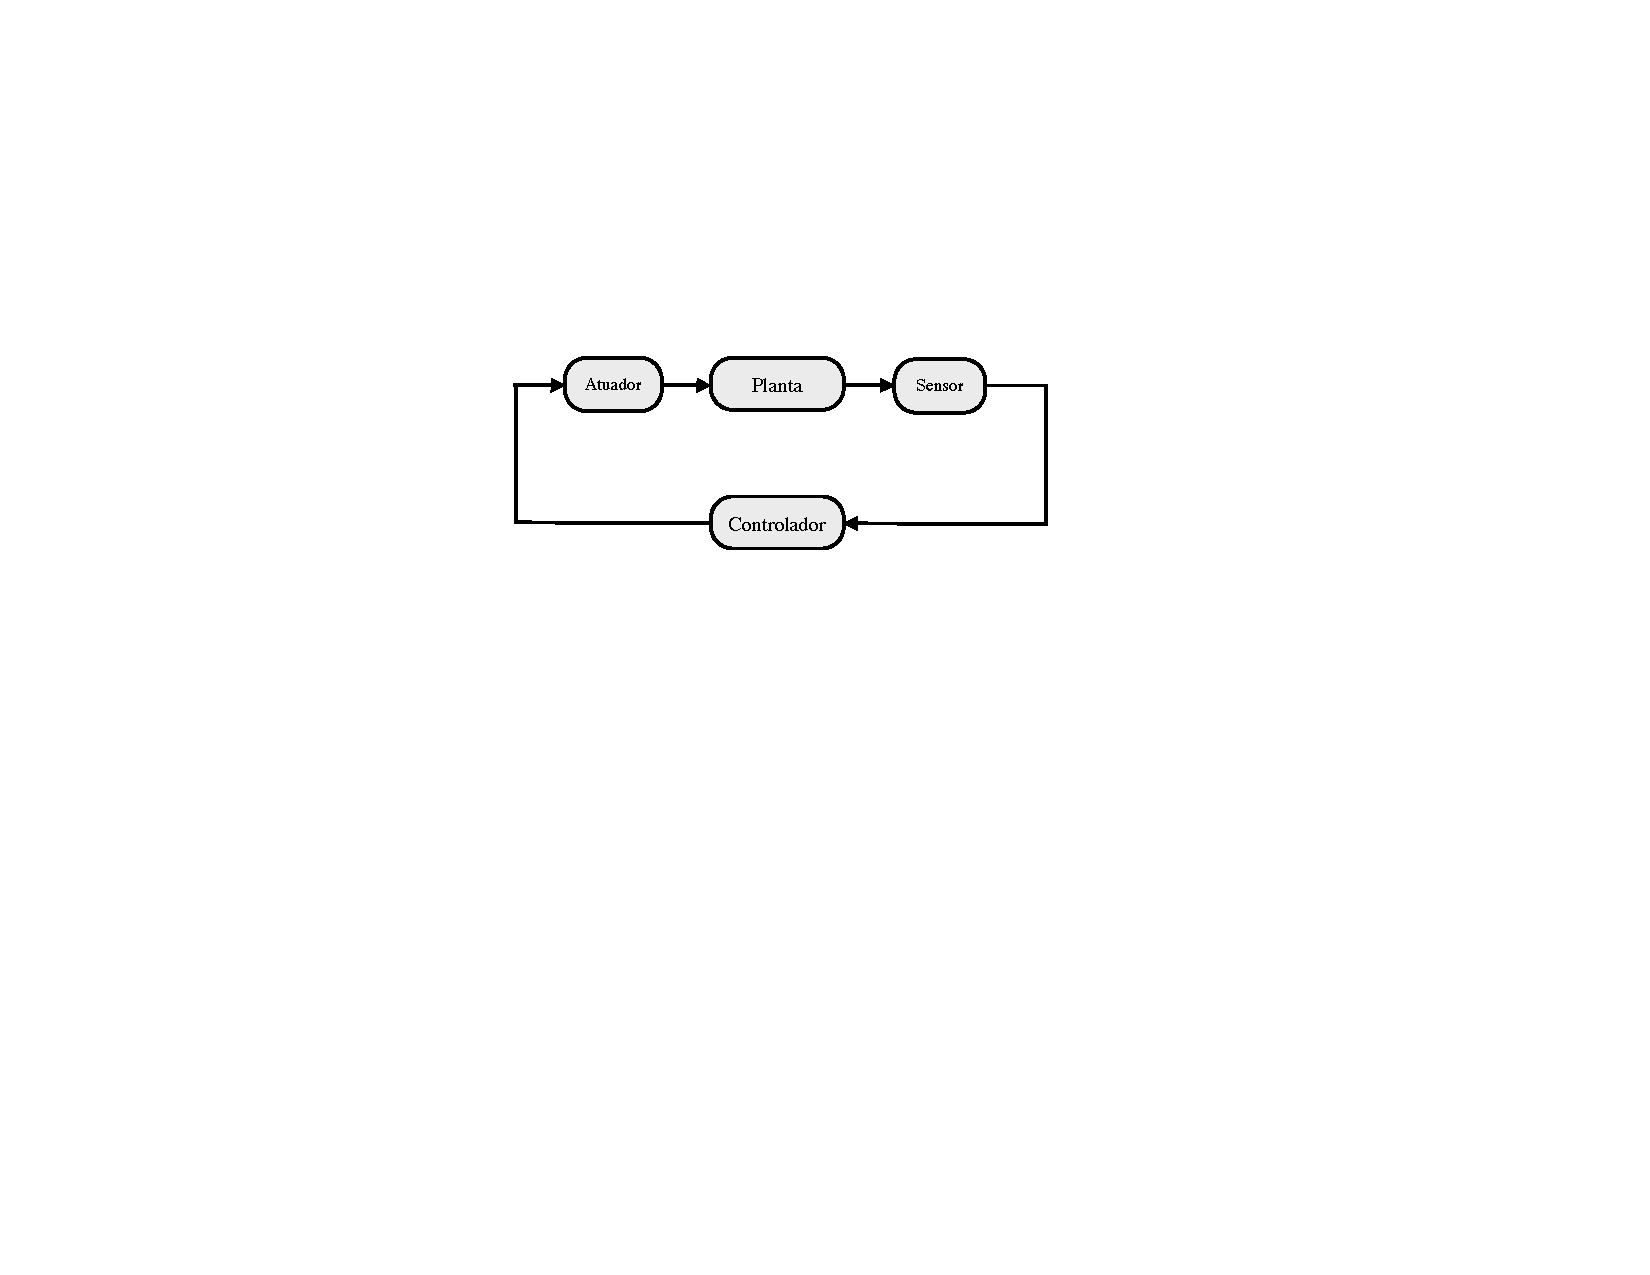
\includegraphics{DescricaoProcesso/Figuras/FiguraProcesso.pdf}}
  \caption{Aqui escrevemos \textbf{toda} informação pertinente à figura. Ou seja, este texto deve ser uma descrição auto-contida da figura, não sendo necessário recorrer ao corpo de texto para saber detalhes sobre a mesma. \emph{Fonte:} Citar fonte se figura 	não for elaborada pelo autor e \textbf{pedir permissão para usar!}}
  \label{fig:processo}
\end{figure}


\section{Situação Atual/Estado da Arte/Revisão da Literatura}
\label{sec:revisão}

Este é o espaço para uma revisão detalhada do enquadramento do problema. Isso inclui descrever a situação atual do processo, aquilo que foi feito até então dentro da empresa/laboratório, e aquilo que se pode chamar de ``Estado da Arte'', ou seja, uma apresentação do conhecimento preexistente
sobre o tema do projeto.

A elaboração desta seção tipicamente demanda uma boa revisão da literatura. Deve haver, quando aplicável uma análise das soluções potencialmente concorrentes, elencando vantagens e desvantagens.

\subsection{Como Elaborar uma Revisão da Literatura}

Ao selecionar referências, devem-se preferir referências de veículos confiáveis, que tenham por exemplo processo de revisão por pares. Portanto, dá-se preferência a artigos em periódicos e livros, em seguida teses e dissertações, artigos em anais de congresso e por fim relatórios. Evitar citar páginas da internet por oferecem menor garantia da informação nelas contida. 

Pesquise sua bibliografia em bases confiáveis como o \textsf{Web of Science}, \textsf{Scopus}, ou o \textsf{Google Scholar}. \textbf{Não use uma ferramenta de busca comum!} (elas não foram feitas pensando no \emph{ranking} de textos científicos) Use o número de citações de uma dada referência como um indicador de sua qualidade. Explore os artigos que citam a referência estudada bem como os artigos que ela cita.

Prefira as referências mais recentes quando se tratar de um assunto na fronteira do conhecimento ou de tecnologia de ponta. Quando se tratar de um assunto já consolidado, prefira citar livros ou artigos com muitas citações. 

Evite citar informações de segunda-mão e procure na medida do possível rastrear a fonte original. Contudo, em situações em que a fonte original é de acesso mais difícil, seja por ter tido publicação limitada como no caso de relatórios ou por não ser em língua inglesa ou portuguesa, é preferível a citação de segunda-mão em um veículo mais acessível.

Para gerenciar suas referências, use uma ferramenta de software como o \textsf{Mendeley}, que permite gerar arquivos .bib para uso em {\LaTeX} ou simplesmente gerar a lista de referências para uso direto em editores de texto. Em \LaTeX, mais especificamente Bib\TeX, a lista de referências é criada a partir de um arquivo .bib, que é uma espécie de banco de informações bibliográficas em que cada entrada é uma referência associada a uma chave para citação. A lista criada incluirá apenas as referências citadas ao longo do texto, mesmo que haja mais referências no arquivo .bib. As informações bibliográficas no formato Bib\TeX também podem ser obtidas para cada referência em ferramentas como o \textsf{Google Scholar} e então coladas no arquivo .bib.

Na Seção \ref{sec:comocitar} discutiremos como e quando as citações devem ser usadas.

\section{Resumo do Capítulo}

Tente não terminar de forma abrupta. Se for escrever algo aqui, não seja genérico!


\clearpage

\chapter{Metodologia}
\label{chap:metodologia}

Este capítulo deve descrever os métodos utilizados no projeto. As teorias e ferramentas utilizadas, assim como as ações executadas, devem ser escritas de forma clara e precisa, sem deixar espaço para ambiguidades. Tenha em mente que \textbf{o objetivo aqui é dar credibilidade ao seu trabalho e permitir que ele possa ser reproduzido por quem tenha interesse (algumas vezes por você mesmo!)}. 

É natural que este capítulo contenha uma revisão bibliográfica mais detalhada das técnicas utilizadas. O ideal é que o capítulo seja auto-contido, de modo que o leitor não necessite recorrer às referências para entender seu trabalho ou reproduzi-lo.

Ao apresentar os métodos, será importante justificar devidamente as opções tomadas e discutir as alternativas disponíveis e os critérios que o levaram à escolha do método.

No restante do capítulo, apresentamos um pequeno manual de escrita técnica.

\section{Técnica 1 - Organização do texto}
\label{sec:metodo1}

Procure \textbf{definir a estrutura} de seu texto \textbf{antes de começar a escrever}. Isso evitará que as ideias apareçam foram de ordem. A falta de organização é uma das características mais comuns de textos difíceis de ler.

Nunca invoque conceitos ou objetos antes de defini-los. Procure fornecer o máximo de informação \emph{a priori} possível. Evite referências para frente no texto. 

Para evitar que o leitor se perca, antes de iniciar um trecho longo de texto que contenha ideias diversas, \textbf{adiante para o leitor o que será feito}, aonde se quer chegar. Ao fim do trecho, declare explicitamente que chegou à conclusão que desejava. Esta técnica vale especialmente para seções e capítulos do texto. 

\section{Técnica 2 - Estilo}
\label{sec:estilo}

O texto técnico deve ser preciso, claro, sem ambiguidades, objetivo e conciso. Mesmo com esse rigor, não deixe de prender a atenção do leitor. Lembre-se de que o início e o fim de cada parágrafo, de cada frase, são as partes mais importantes e onde você deve colocar maior ênfase.


\subsection{Precisão}

Use as palavras corretas! Não escreva redondo se é esférico. Não escreva igual se é aproximado. Não escreva sistema se é função de transferência. Não escreva grande, pequeno, máximo, mínimo, ótimo, se não há uma escala que defina tais conceitos.

Prefira usar números que deem uma noção de escala a usar adjetivos difíceis de precisar.

Seja específico e evite generalidades. Por exemplo, em vez de dizer ``O processo 1 é um processo de alto custo'', devemos ser mais precisos com relação à natureza do custo e dizer ``O processo 1 possui custo operacional elevado com relação a processos tradicionais tais como o processo 2''.

\subsection{Clareza}

Não deixe margem para dúvidas! Para reduzir a possibilidade de confusão na leitura do seu texto, \textbf{evite frases longas}. Nunca escreva frases com mais de $20$ palavras. Procure escrever na média $12$ palavras por frase. Evite palavras compridas ou que possam ser consideradas difíceis.

Não deixe ideias subentendidas! Não assuma que seu leitor pensa como você e vai saber do que você está falando. Explicite todos os passos de seu raciocínio lógico. Pular passos de raciocínio é uma das causas mais comuns de confusão na leitura. Não seja preguiçoso neste quesito.

Novamente, defina todos os conceitos antes de fazer uso deles.

Não deixe o sujeito verbal subentendido. Para evitar ambiguidades, tome cuidado ao usar pronomes como ``esse, este, isso, ele''. É preferível repetir um nome a deixar margem para dúvidas. Por exemplo, após a primeira frase deste parágrafo poderíamos dizer de forma não tão clara: ``Esta é uma causa de confusão na escrita.''; ou poderíamos dizer de forma mais clara: ``Essa falta de informação é uma causa de confusão na escrita.''

Não há problemas em haver repetições em textos técnicos. O mais importante é a clareza, a inexistência de ambiguidades, não a beleza. Se acha que uma determinada frase pode ser confusa ou se alguma ideia parece difícil de explicar, repita a mesma ideia em outras palavras ou, melhor ainda, dê um exemplo.

Por fim, domine o significado das palavras utilizadas para evitar ambiguidades. Se uma palavra pode ter mais de um significado em determinada frase, tente trocá-la por outra que não deixe dúvidas. Mais importante ainda, não use palavras sobre cuja definição você não tem certeza.

\subsection{Ojetividade}

O texto técnico deve ser direto ao ponto, sem rodeios, e livre de opiniões. Evite apartes, evite divagações e discussões irrelevantes com relação ao tema principal.

\textbf{Nunca use hipérboles}. Cuidado com termos como ``otimizar, muito grande, enorme, muito bom''.  Usar números sempre que possível para quantificar conceitos, sejam eles precisos ou apenas uma estimativa. Em especial deve-se tomar cuidado com as palavras ``muito'' e ``muitos''.

O tom deve ser impessoal, apresentando apenas fatos e não opiniões. Em português, a voz passiva é um instrumento comum para se obter um tom impessoal. Contudo, sempre que possível, tente usar a voz ativa ou a voz passiva sintética para deixar o texto mais fluido e claro.

Palavras abstratas deixam a escrita vaga. Prefira palavras concretas, fortes, isto é, palavras que tenham um único significado. Sempre que possível substitua múltiplas palavras por uma única. Por exemplo, na frase ``A máquina processou as amostras'' temos duas palavras genéricas: máquina e processar. A mesma ideia seria mais objetiva se expressa como ``A centrífuga girou as amostras''.

Controle seu tom. \textbf{Não use linguagem coloquial. Não use clichês}. Não use de arrogância: ``obviamente, como é sabido, é claro que''. 

\subsection{Concisão}

O texto técnico deve ser tão curto quanto possível, sem prejuízo de sua clareza e precisão. Não use palavras a mais, não inclua expressões irrelevantes ou supérfluas. Não escreva simplesmente para encher as páginas. Se um assunto não é relevante para a compreensão do seu trabalho, corte-o, mova-o para um apêndice ou aponte uma referência.

Evite redundâncias como ``opinião pessoal'' e ``garantia absoluta''.

\section{Vícios comuns}

\begin{itemize}
\item Estrangeirismos: ``\emph{performance}'', ``\emph{mutatis mutandis}''. Se necessário, coloque o termo estrangeiro em itálico e dê uma tradução entre parênteses.

\item Usar linguagem rebuscada. Lembre-se de que a linguagem técnica deve ser clara, precisa e objetiva.

\item Alternar o tempo verbal entre passado e presente. Seja consistente e escreva apenas no passado ou no presente.

\item Iniciar uma frase com verbo porque o sujeito está implícito na frase anterior. Deixe sempre o sujeito explícito.

\item Inserir referências no meio de uma frase. Isso quebra o fluxo da leitura. Coloque a citação no fim da frase.

\item \textbf{Usar siglas sem antes defini-las}. Sempre escreva a sigla por extenso \emph{na primeira vez} que ela aparece no texto. Por exemplo, ``este é um texto de Projeto Final de Curso (PFC)''. 

\item Escrever ``como sabemos'', ``como é sabido'', ``por razões óbvias'', ``é evidente que'', ``talvez seja verdade que''. Estes termos significam apenas que você não sabe explicar o que está afirmando.

\item Usar definições \emph{por exemplo}, isto é, apresentar a definição de um conceito ou termo por meio de um exemplo. Primeiro defina o conceito, depois exemplifique.

\end{itemize}

\section{Boas práticas}

\begin{itemize}
\item Sempre que introduzir novos termos e conceitos, destaque-os em itálico para que o leitor saiba que se trata de uma definição e para que ele ache a definição com facilidade quando for necessário rastreá-la no texto.
\item Releia o que escreve a cada parágrafo. Releia rapidamente cada seção para verificar o encadeamento de ideias.
\item Corte palavras sempre que possível.
\item Nunca assuma que o leitor entenderá o que você escrever. Esforce-se para fazê-lo entender.
\item Use um corretor ortográfico.
\item Peça que alguém leia seu texto.
\end{itemize}


\section{Uso de referências}
\label{sec:comocitar}

Uma afirmação incluída num texto técnico se enquadra em um de três casos: a) seu conteúdo é de conhecimento geral dentro da área do texto; b) seu conteúdo é original e resulta do trabalho do autor; c) seu conteúdo tem origem em outro trabalho (ainda que seja do mesmo autor, não é original).

Toda afirmação enquadrada na categoria c) deve ser acompanhada de uma citação. Para afirmações da categoria b), deixe claro que se trata de ideia original do autor. Isso evita que o leitor se confunda ao pensar que possa se tratar de a) ou c).

No caso a), pode ser um tanto mais sutil determinar o que deve ser de conhecimento geral. Procure evitar o excesso de citações. Se todo um parágrafo se baseia em ideias de uma certa referência, em geral basta que ela seja citada no seu início.

\textbf{Atenção:} Não copie frases das referências usadas. Reescreva as ideias com suas próprias palavras e não deixe de citar a fonte. Se for necessário manter as palavras do original, cite a frase entre aspas e em itálico.

\section{Honestidade e Plágio}

Seja honesto ao escrever. \textbf{Não ``maqueie'' seus resultados}. Não apresente apenas as melhores amostras dos seus resultados para dar a impressão de que foi bem sucedido. Não escreva aquilo que não entende. Não escreva de forma vaga para mascarar o fato de que não entende algo.

Dê crédito a quem o merece. Inclua referências sempre que usar o trabalho de outros. Seja sempre claro para não dar a impressão de que fez algo feito por outrem. \textbf{Não assuma crédito pelo trabalho dos outros}. Isso pode ter implicações legais e acadêmicas.

\section{Cuidado com a gramática}

\begin{itemize}

\item Erros gramaticais deixam uma \textbf{impressão ruim} e podem alterar a disposição do leitor para com o texto.  

\item Use a vírgula corretamente. Seu uso incorreto confunde o leitor. Nunca use a vírgula porque acha que a frase precisa de uma pausa. Não separe sujeito e verbo. Quando há inversão da ordem natural em uma frase, \emph{toda} a parte movida deve estar entre vírgulas.

\item Cuidado com a concordância da voz passiva sintética. Lembre-se de que o correto é ``Vendem-se ovos'' e não ``Vende-se ovos''.

\item Use a crase corretamente. Faça sempre o exercício de substituir o nome que sucede o ``à'' por um nome no masculino. Se o correto for usar ``ao'' com o nome masculino, então deve haver crase. Nunca use crase antes de nomes no masculino!

\item Escreva ``em que'' em vez de ``onde'' quando não houver indicação de lugar.

\item Não se escreve ``o fato \textbf{dela} ser'' ou ``a razão \textbf{do} texto ser escrito''. Escreve-se ``o fato \textbf{de ela} ser'' e ``a razão \textbf{de o} texto ser escrito''.

\item Releia o que escreve e na dúvida busque ajuda.

\end{itemize}

\section{Resumo do Capítulo}
\label{sec:metodo1b}

Tente não terminar de forma abrupta. Se for escrever algo aqui, não seja genérico!


\clearpage
\chapter{Resultados}

Para a execução do projeto, algumas etapas de desenvolvimento tiveram de ser seguidas: familiarização com o sistema, estudo dos módulos envolvidos, leitura dos requisitos, elaboração de documento descrevendo todo o processo de implementação e relacionamento com os diversos módulos, implementação e testes.


\section{Atividades do Projeto}
\label{metodo3}

\section {Requisitos do Sistema}
\label{req}


\section{Desenvolvimeto e Implementação}

A Tabela \ref{tab:tabela} apresenta as atividades executadas.

\begin{table}
\centering
%Note os alinhamentos diferentes em cada coluna
\begin{tabular}{|c|r|l|}\hline
		Atividade 1 & aa  & ab  \\ 
					 & a & b \\ \hline
		Ativ. 2  & aa & ab \\			
					 &  a & b \\ \hline
		\end{tabular}
	\caption{Exemplo de tabela - Coloque toda informação sobre a tabela aqui}
	\label{tab:tabela}
\end{table}

\section{Testes}

\section{Análise dos Resultados}

Apresente os resultados sem adulterações e faça análises objetivas. Pense na melhor maneira de apresentar os resultados graficamente. Se os gráficos são difíceis de interpretar, talvez tabelas sejam uma forma melhor de apresentar resultados. Não apresente dados (gráficos e tabelas) se não há uma conclusão interessante a ser tirada. Lembre-se de ser conciso.

\emph{Não se esqueça das unidades!} Pense que \emph{a priori} todo número deve ter uma unidade. Não escreva as unidades em itálico (no ambiente matemático) e tome cuidado para diferenciar maiúsculas e minúsculas. Um exemplo é escrever $22$ [kN] e não $22 KN$ (Kelvin vezes Newton!).

Ao apresentar resultados experimentais, tome o cuidado para também apresentar o cálculo das incertezas sempre que forem significativas. Ao fazer conclusões, sempre considere se o tamanho da sua amostra é grande o suficiente do ponto de vista estatístico. Lembre que a média empírica $\hat{\mu}_X$ de $N$ observações independentes da variável $X_i$ possui variância
\[
\hat{\sigma}_{\mu}^2 = \frac{1}{N(N-1)} \sum_{i=1}^N (X_i-\hat{\mu}_X)^2
\enspace,
\]
onde se assume que as variáveis $X_i$ possuem uma mesma ditribuição e que essa distribuição possui segundo momento finito.


\section{Resumo do Capítulo}
\label{sec:resumoo4}
Tente não terminar de forma abrupta. Se for escrever algo aqui, não seja genérico!

\section{Formato, expressões matemáticas e o \LaTeX}

\subsection{O \LaTeX}

O {\LaTeX}  é o método preferencial de preparação de documentos para textos técnicos nas ciências exatas. O {\LaTeX} permite não só lidar com equações de uma forma mais prática que em editores de texto, mas também facilita a formatação de documentos e tem um desempenho marcadamente superior a editores de texto na preparação de documentos longos como monografias. 

Documentos em {\LaTeX} são escritos em um ou mais arquivos de texto com extensão .tex. Após a escrita, o .tex é \emph{compilado} para gerar arquivos nos formatos .pdf, .dvi ou .ps. Hoje há duas distribuições padrão para o \LaTeX. Sistemas Windows usam o {Mik\TeX} e sistemas Unix usam o \TeX Live. Além das distribuições, muitos usuários utilizam \emph{front-ends} que facilitam a edição do texto, a compilação e a instalação de pacotes. 

Os pacotes necessários para compilar o presente documento devem ser encontrados numa instalação completa dessas distribuições. Se tiver dificuldades com os pacotes, você pode instalá-los manualmente ou tentar alterar o código para usar versões antigas dos mesmos.

A compilação pode ser feita pelos comandos \textsf{latex} ou \textsf{pdflatex}, invocados pela linha de comando ou pelo \emph{front-end}. Note que será necessário empregar o comando \textbf{mais de uma vez} para que as referências cruzadas saiam corretas.

Como discutido na Seção \ref{sec:revisão}, uma ferramenta útil para gerenciar as citações em {\LaTeX} é o Bib\TeX. Para gerar uma lista bibliográfica a partir do arquivo .bib, este arquivo deve ser indicado no arquivo .tex. Em seguida devem-se executar os comandos \textsf{pdflatex}, \textsf{bibtex} e \textsf{pdflatex} novamente sempre usando o .tex como argumento. Note que os comandos são executados nesta ordem e de forma repetida para que as referências cruzadas sejam geradas corretamente.

Nesta seção você deve encontrar exemplos dos comandos mais usados em \LaTeX. Outros exemplos e manuais podem ser encontrados na internet com facilidade.

\subsection{Expressões Matemáticas}

Ao escrever expressões matemáticas, defina todas as variáveis antes de usá-las ou imediatamente depois da expressão. Deixar de fazê-lo torna seu texto \textbf{ilegível}. Segue um exemplo.

Seja o par $(a_1,a_2)\in \mathbb{R}^2$. Para $s\in\mathbb{C}$, definimos a função $f(s)$ como
\[%cria equações sem numeração
f(s)\triangleq \frac{a_1 s+a_2}{s^2+2\zeta\omega_n s+\omega_n^2}
\enspace,
\]
onde os escalares $\zeta,\omega_n>0$ são constantes.

Note que não foi necessário atribuir valores às variáveis neste momento. Repare também como devemos \textbf{usar pontuação} (vírgula) nas equações, tratando-as como parte da frase. Usamos o símbolo $\triangleq$ ou $:=$ para deixar explícito que se trata de uma definição. Ser claro nesse aspecto facilita o entendimento do leitor.

A equação acima não foi numerada porque não será citada no texto. Vejamos um exemplo com numeração.

A função $f(\cdot)$ possui um zero em $-a_2/a_1$ (ou $-\frac{a_2}{a_1}$) e, para $\zeta<1$, possui polos complexos $p_{1,2}$ dados por
\begin{equation}
\label{eq:polos}
p_{1,2}=\omega_n \left(-\zeta\pm j\sqrt{1-\zeta^2}\right)
\enspace.
\end{equation}
Agora podemos citar os polos dados pela Equação (\ref{eq:polos}) (aqui adotamos a convenção de citar sempre com o número entre parênteses precedido da palavra Equação). Note como usamos um comando especial na Equação \ref{eq:polos} para garantir o ajuste automático do tamanho dos parênteses.

Vejamos agora como criar equações alinhadas. Considere o sistema dinâmico dado pelas equações diferenciais:

\begin{align}
\dot{x}_1 & = \cos(x_2)\cdot\ln(1/x_1)+\tan(u) \label{eq:x1dot} \\
\dot{x}_2 & = e^{-x_1-x_2} \nonumber \\
& y  = \min\{x_1,x_2\}  \label{eq:saida}
\enspace,
\end{align}
onde $x(t)=[x_1(t) ~ x_2(t)]'$, $t>0$, é a variável de estado do sistema, $u(t)$ é o sinal de entrada e $y(t)$ é o sinal de saída do sistema. Note no .tex que o caracter de tabulação \textsf{\&} foi usado para indicar o ponto de alinhamento horizontal das equações. Além disso, para ilustrar o uso do \LaTeX, retiramos a numeração da segunda equação e citamos as equações separadamente.

Nas Equações (\ref{eq:x1dot}) e (\ref{eq:saida}), aparecem operadores como $\min$, $\ln$, $\cos$ e $\tan$. A convenção aqui é que \textbf{variáveis devem ser escritas em itálico e operadores não}. Por essa razão todas as expressões matemáticas devem ser escritas no ambiente matemático (entre cifrão) mesmo quando for possível usar texto comum. Isso garante a consistência das fontes utilizadas (nem sempre a fonte do ambiente matemático é a mesma fonte do texto). 

Para escrever matrizes, podemos fazer por exemplo:
\[
\sum_{n=0}^{\infty}z^{-n}\left[\begin{array}{cc}
\lambda & 1 \\
0 & \lambda
\end{array}\right]^n=
\left[\begin{array}{cc}
\frac{z}{z-\lambda} & \frac{z}{(z-\lambda)^2} \\
0 & \frac{z}{z-\lambda}
\end{array}\right]
,~\forall \lambda<|z|
\enspace.
\]

Para escrever uma expressão com múltiplos casos, podemos fazer, para um inteiro $N$ positivo,
\[
g[n]=
\left\{
\begin{array}{ll}
0,& \mbox{se }~ n\leq 0 \\
n,& \mbox{se }~ n=1,2,\ldots,N-1 \\
N,& \mbox{se }~ n\mod N = 0 \\
0,& \mbox{caso contrário}\enspace.
\end{array}
\right.
\]

\textbf{Nunca reaproveite símbolos} matemáticos, isto é, nunca use o mesmo símbolo para designar variáveis diferentes.

Para um exemplo com múltiplas linhas de expressão matemática: tem-se que, para $a\neq 0$,

\begin{equation}
\begin{split}
ax^2+bx+c &= 0 \\
& \Rightarrow a(x^2+bx/a+c/a) =0 \Rightarrow a((x+b/(2a))^2+c/a-b^2/(4a^2))=0  \\
& \Rightarrow (x+b/(2a))^2=(b^2-4ac)/(4a^2) \\
& \Rightarrow (x+b/(2a))=\pm\sqrt{b^2-4ac}/(2a) \\
& \Rightarrow x=\frac{-b\pm\sqrt{b^2-4ac}}{2a}
\enspace.
\end{split}
\end{equation}

Note a argumentação lógica aqui. Não estamos dizendo que o valor de $x$ é dado pela última linha. Estamos dizendo que a hipótese da primeira linha juntamente com a hipótese $a\neq 0$ implicam os referidos valores de $x$. \textbf{Um erro comum dos alunos ao escrever é não distinguir a veracidade das implicações com a veracidade das hipóteses}.

\clearpage
\chapter{Conclusões}

\section{Considerações Finais}

Aqui vai o texto da conclusão.

\section{Propostas de Continuidade}


\clearpage


\addcontentsline{toc}{chapter}{Referências Bibliográficas}
\renewcommand{\bibname}{Referências Bibliográficas}

%\bibliographystyle{abntex2-alf} %para norma ABNT no sistema autor-data
\bibliographystyle{abntex2-num}
\begin{small}
\bibliography{ListadeReferencias}%,library}
%% Monografia para Projeto de Fim de Curso - Exemplo no LaTeX
%-----------------------------------------------------------


%---------------Inicialização de pacotes--------------------

\documentclass[12pt,a4paper,notitlepage,twoside]{book}


\usepackage{graphicx}
\usepackage[utf8]{inputenc}
%\usepackage[latin1]{inputenc} %%pode ser necessário trocar a codificação em sistemas Windows
\usepackage[brazil]{babel}		%%pode ser necessário trocar o pacote de línguas em algumas distribuições LateX
%\usepackage[portuguese]{babel}
\usepackage[T1]{fontenc}
\usepackage{amsmath,amssymb}
\usepackage{amsthm,amsfonts}
\usepackage{color}
\usepackage[colorlinks]{hyperref}
\usepackage{abntex2abrev}
%\usepackage[alf]{abntex2cite} %se você quiser seguir as normas ABNT no sistema autor-data
%\usepackage[num]{abntex2cite} %se você quiser seguir as normas ABNT no sistema numérico
\usepackage{setspace}
\usepackage[toc,page]{appendix}

%Definindo fonte Times (Use os pacotes obsoletos se não conseguir instalar os atualizados)
%\usepackage{times}     %Pacote de fontes obsoleto, apenas texto
%usepackage{mathptmx}  %Pacote de fontes obsoleto, texto e símbolos matemáticos
%\usepackage{newtxtext,newtxmath}  %Pacotes de fontes mais recentes

\usepackage[a4paper,top=30mm,bottom=30mm,inner=30mm,outer=25mm,headheight=7mm,headsep=6mm,footskip=7mm]{geometry}
\usepackage{enumerate}

\makeindex

%\singlespacing   %%espaçamento simples
%\onehalfspacing
%\setstretch{1.03} %%um pouco melhor que espaçamento simples
\linespread{1.25} %corresponde ao espaçamento 1.5 do MS Word

%---------------Início do documento-------------------------

\begin{document}

\begin{titlepage}
\begin{center}
{\large Universidade Federal de Minas Gerais\\
Escola de Engenharia \\
Curso de Graduação em Engenharia de Controle e Automação\\}

\vspace{6cm}
{\bf\Large Primeira Linha do Título\vspace{0.2cm}

Segunda Linha do Título, se Houver}
\vspace{4cm}

%\hspace{0.3\textwidth} \parbox{0.65\textwidth}
{\large André Sales Barbosa}
\vspace{2cm}  
   
\vspace{2cm}          
%\hspace{0.3\textwidth} 
{\large Orientador: Prof. Antônio de Pádua Braga, Dr.}\\


\vfill
%\hspace{0.3\textwidth} 
{\large Belo Horizonte, Dezembro de 2017 }
\end{center}

\end{titlepage}

\newpage
\clearpage
\thispagestyle{empty}


\begin{titlepage}

\centering
\textbf{Monografia}\\
\vspace{2cm}
\centering
\textbf{Título da Monografia}\\
\vspace{5cm} 

\parbox{1.0\textwidth} 
{\large 
Monografia submetida à banca examinadora
designada pelo Colegiado Didático do Curso de
Graduação em Engenharia de Controle e
Automação da Universidade Federal de Minas
Gerais, como parte dos requisitos para aprovação na
disciplina Projeto Final de Curso II.}

\vspace{7cm} 
\centering
Belo Horizonte, Dezembro de 2017

\end{titlepage}

\clearpage
\thispagestyle{empty}
\cleardoublepage

\pagenumbering{roman}
\section{Descrição do problema e solução proposta}

Esse trabalho de projeto de final de curso se dedica à implementação do algoritmo
 de reconhecimento de padrões para classificar movimentos.
Para isso faz-se o uso de uma placa de desenvolvimento do  microcontrolador ESP32 e um sensor 
acelerômetro MPU6050. O protótipo desenvolvido deverá reconhecer qual movimento foi aplicado
 ao objeto e exercer uma atuação a partir disso.
 A inspiração para o projeto veio do conceito de inteligência distribuída. Nessa abordagem o
 algoritmo de inteligência artificial é implementado nos dispositivos de borda ("edge"), evitando
 a transferência de dados para um processamento central.

\addcontentsline{toc}{chapter}{Abstract}

\begin{center}
\huge{{\bf Abstract}}
\vspace{2cm}
\end{center}

Write a version of your ``resumo'' in English. Beware of literal translations and double check the translation of technical terms.
 

 
\clearpage
\thispagestyle{empty}
\cleardoublepage


\addcontentsline{toc}{chapter}{Agradecimentos}

\begin{center}
\huge{{\bf Agradecimentos}}
\vspace{4cm}
\end{center}

Aqui vai o texto dos agradecimentos.
 
\clearpage
\thispagestyle{empty}
\cleardoublepage
\tableofcontents
%\markboth{Conteúdo}{Conteúdo}

\clearpage
%\thispagestyle{empty}
%\cleardoublepage

% Normalmente, este arquivo só contém isto.
\listoffigures
\addcontentsline{toc}{chapter}{Lista de Figuras}
%\markboth{Lista de Figuras}{Lista de Figuras}

\clearpage
%\thispagestyle{empty}
%\cleardoublepage

% Normalmente, este arquivo só contém isto.
\listoftables
\addcontentsline{toc}{chapter}{Lista de Tabelas}
%\markboth{Lista de Tabelas}{Lista de Tabelas}

\clearpage
%\thispagestyle{empty}
%\cleardoublepage

% Normalmente, este arquivo só contém isto.

\pagenumbering{arabic}
\setcounter{page}{1}
\chapter{Introdução}
%\markboth{\thechapter ~~~ Introdução}{}
%\label{intro}

Se preferir, você pode apresentar este Capítulo antes da primeira Seção, destacando os principais pontos que são abordados. %\cite{Raffo2008}

\section{Motivação e Justificativa}
\markright{\thesection ~~~ Motivação}
%\label{motiva}


\section{Objetivos do Projeto}
\markright{\thesection ~~~ Objetivos}
%label{objetivos}

Tendo em vista o exposto acima, este projeto tem por objetivos:

\begin{itemize}
\item[a.] Item 1;
\item[b.] Item 2;
\item Etc.
\end{itemize}




\section{Local de Realização}
\markright{\thesection ~~~ A Empresa}
%\label{empresa}

Vale à pena descrever a empresa onde o PFC foi desenvolvido. Veja o exemplo abaixo.

O projeto de fim de curso foi desenvolvido na empresa ..., no Departamento de ..., responsável por toda a implementação do sistema de ...

A empresa realiza projetos de pesquisa e desenvolvimento, consultoria e treinamento nas áreas de ...

A ... foi criada em ...  

A empresa é divida em três departamentos: (o arquivo Introducao.tex mostra como criar a lista abaixo) 

\begin{itemize}
\item Departamento de ... 
\item Departamento de ...
\item Departamento de ...
\end{itemize}

Este projeto foi desenvolvido no Departamento de ..., que é o responsável por ...

Os demais Departamentos englobam as fun\c{c}\~oes de ...

Todos os departamentos trabalham em conjunto. O Departamento de ..., por exemplo, precisa manter um grande vínculo com o Departamento de ... Isso ocorre porque todas as especifica\c{c}\~oes de hardware e sistemas influenciam a forma de implementa\c{c}ão de servi\c{c}os, organiza\c{c}\~ao de tabelas e recursos disponíveis.




\section{Estrutura da Monografia}
\markright{\thesection ~~~ Organização do Trabalho}
%\label{organiza}

O trabalho está dividido em quatro capítulos. Este capítulo apresentou uma introdução ao projeto a ser descrito nesta monografia e a empresa onde o trabalho foi realizado. O Capítulo 2 descreve os princípios básicos de um sistema ... (sistema onde se insere o trabalho) e abrange todos os conceitos necessários para um melhor entendimento do projeto. O Capítulo 3 aborda a metodologia de desenvolvimento, seguida pela implementa\c{c}\~ao dos .... No Capítulo 4 tem-se a conclusão da  monografia e algumas sugest \~oes e dificuldades encontradas na realização do projeto.


\clearpage
\chapter[Descrição do Processo]{Descrição do Problema/Processo ou O Processo de Fazer Alguma Coisa}
\label{chap:descricaoproblema}
%Note que, como nome do capítulo é muito longo, fornecemos um nome abreviado uso no cabeçalho

Se desejar, uma visão geral do capítulo pode ser colocada antes da primeira seção. Este é o capítulo de descrição do processo e formulação do problema. Tendo em vista que se trata de uma monografia de engenharia de controle e automação, em muitos casos será fundamental a apresentação dos sensores e atuadores do processo.


\section{Processo de Fazer Alguma Coisa}
\label{sec:hist}

Cada seção inicia pela descrição do seu conteúdo e pode terminar com um parágrafo de conexão com a seção seguinte. 

Antes de formular o problema, \textbf{não se esqueça de fazer todas as definições necessárias}. Também devem-se detalhar os aspectos complementares da abordagem: se estamos estudando um aspeto particular do problema, se a resposta encontrada é universal ou dependente de simplificações e hipóteses prévias.


\section{Instrumentação do Processo}
\label{sec:instrumentação}

Descreva a aparelhagem e o equipamento utilizados bem como a ligação entre os diversos componentes. Nesta seção e, ao longo de todo o texto, você deve dar detalhes suficientes para que qualquer pessoa consiga reproduzir seus experimentos.

Contudo, \textbf{não disperse o leitor com detalhes irrelevantes} ou aspectos
demasiado técnicos ou formais. Reserve tais detalhes para um
apêndice.

Como uma imagem vale mais que mil palavras, e como usar mil palavras prejudicaria a clareza do texto, ilustramos o processo com a Figura \ref{fig:processo}. Lembrar que toda figura deve ser comentada no texto, você nunca deve colocar figuras que fiquem ``soltas'' no texto.  

\begin{figure}[thpb]
  \centering
  \resizebox{120mm}{!}{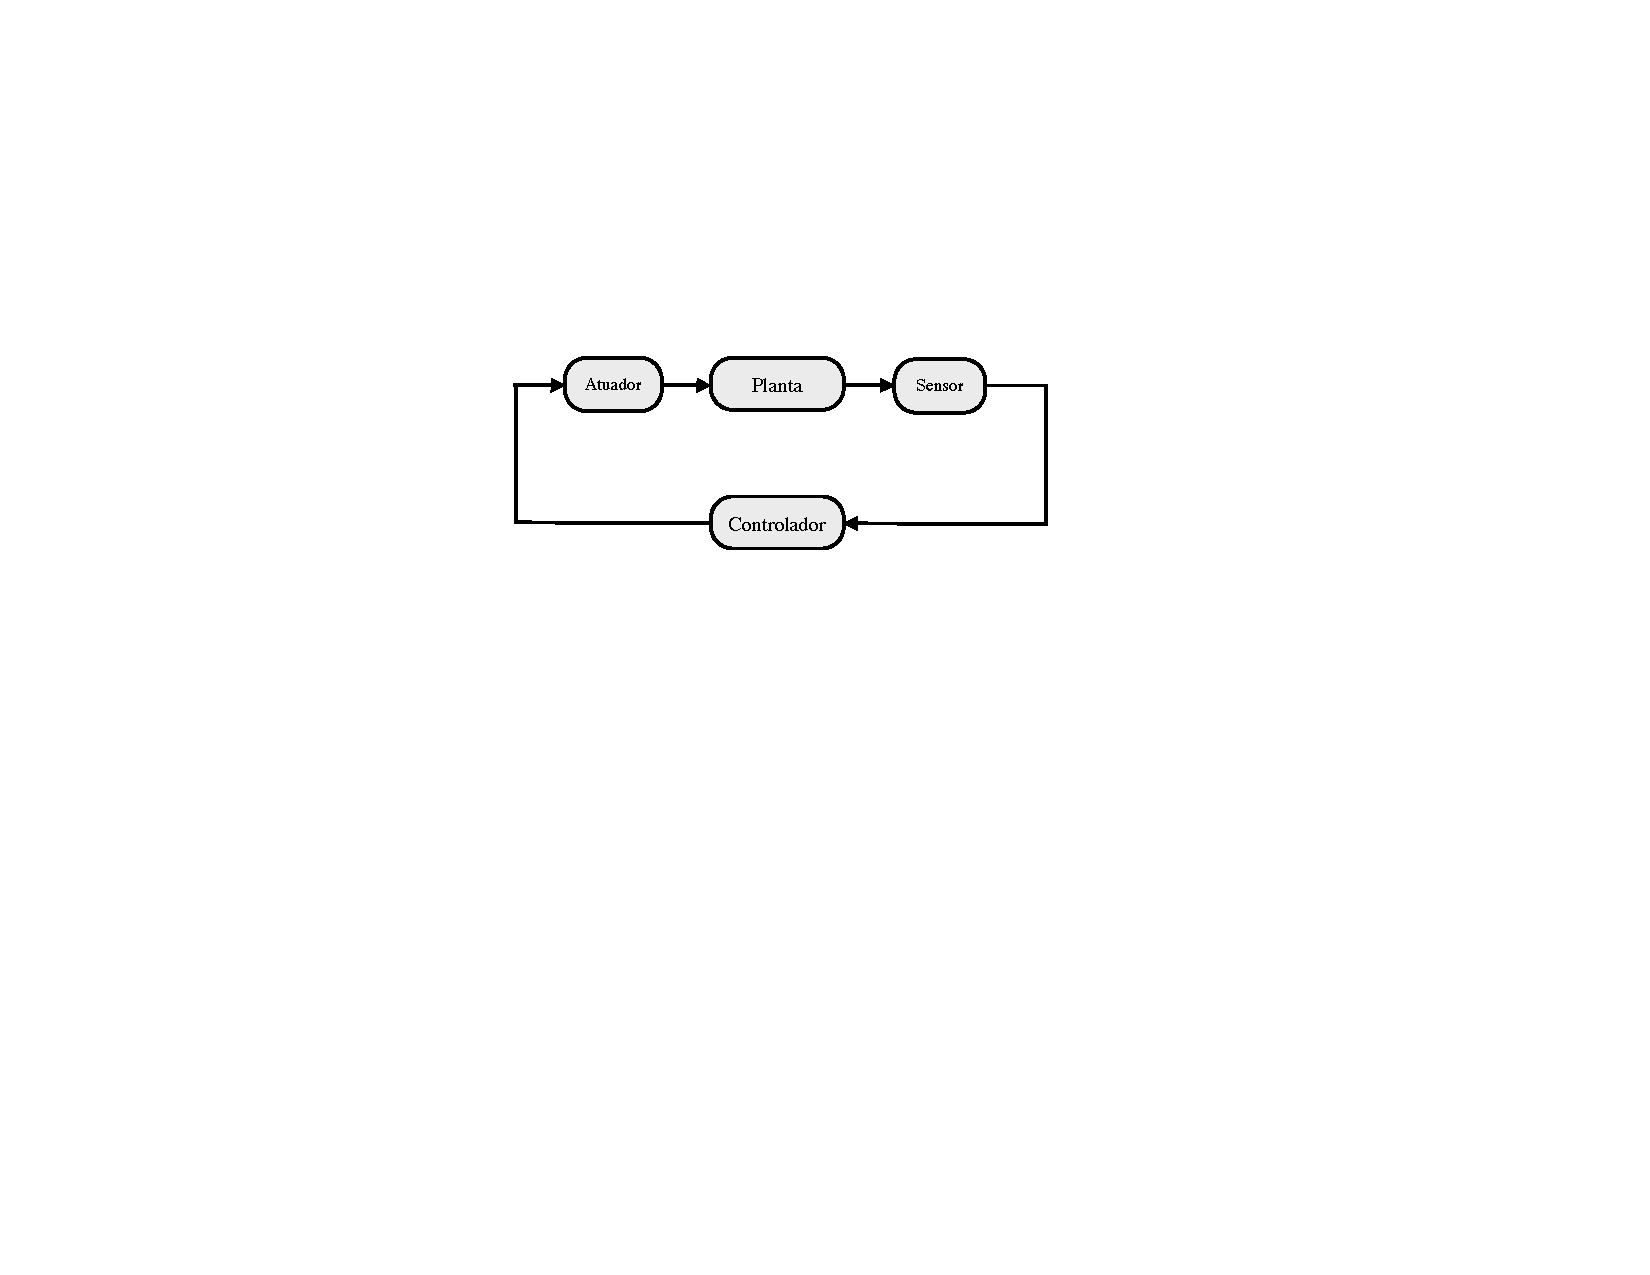
\includegraphics{DescricaoProcesso/Figuras/FiguraProcesso.pdf}}
  \caption{Aqui escrevemos \textbf{toda} informação pertinente à figura. Ou seja, este texto deve ser uma descrição auto-contida da figura, não sendo necessário recorrer ao corpo de texto para saber detalhes sobre a mesma. \emph{Fonte:} Citar fonte se figura 	não for elaborada pelo autor e \textbf{pedir permissão para usar!}}
  \label{fig:processo}
\end{figure}


\section{Situação Atual/Estado da Arte/Revisão da Literatura}
\label{sec:revisão}

Este é o espaço para uma revisão detalhada do enquadramento do problema. Isso inclui descrever a situação atual do processo, aquilo que foi feito até então dentro da empresa/laboratório, e aquilo que se pode chamar de ``Estado da Arte'', ou seja, uma apresentação do conhecimento preexistente
sobre o tema do projeto.

A elaboração desta seção tipicamente demanda uma boa revisão da literatura. Deve haver, quando aplicável uma análise das soluções potencialmente concorrentes, elencando vantagens e desvantagens.

\subsection{Como Elaborar uma Revisão da Literatura}

Ao selecionar referências, devem-se preferir referências de veículos confiáveis, que tenham por exemplo processo de revisão por pares. Portanto, dá-se preferência a artigos em periódicos e livros, em seguida teses e dissertações, artigos em anais de congresso e por fim relatórios. Evitar citar páginas da internet por oferecem menor garantia da informação nelas contida. 

Pesquise sua bibliografia em bases confiáveis como o \textsf{Web of Science}, \textsf{Scopus}, ou o \textsf{Google Scholar}. \textbf{Não use uma ferramenta de busca comum!} (elas não foram feitas pensando no \emph{ranking} de textos científicos) Use o número de citações de uma dada referência como um indicador de sua qualidade. Explore os artigos que citam a referência estudada bem como os artigos que ela cita.

Prefira as referências mais recentes quando se tratar de um assunto na fronteira do conhecimento ou de tecnologia de ponta. Quando se tratar de um assunto já consolidado, prefira citar livros ou artigos com muitas citações. 

Evite citar informações de segunda-mão e procure na medida do possível rastrear a fonte original. Contudo, em situações em que a fonte original é de acesso mais difícil, seja por ter tido publicação limitada como no caso de relatórios ou por não ser em língua inglesa ou portuguesa, é preferível a citação de segunda-mão em um veículo mais acessível.

Para gerenciar suas referências, use uma ferramenta de software como o \textsf{Mendeley}, que permite gerar arquivos .bib para uso em {\LaTeX} ou simplesmente gerar a lista de referências para uso direto em editores de texto. Em \LaTeX, mais especificamente Bib\TeX, a lista de referências é criada a partir de um arquivo .bib, que é uma espécie de banco de informações bibliográficas em que cada entrada é uma referência associada a uma chave para citação. A lista criada incluirá apenas as referências citadas ao longo do texto, mesmo que haja mais referências no arquivo .bib. As informações bibliográficas no formato Bib\TeX também podem ser obtidas para cada referência em ferramentas como o \textsf{Google Scholar} e então coladas no arquivo .bib.

Na Seção \ref{sec:comocitar} discutiremos como e quando as citações devem ser usadas.

\section{Resumo do Capítulo}

Tente não terminar de forma abrupta. Se for escrever algo aqui, não seja genérico!


\clearpage

\chapter{Metodologia}
\label{chap:metodologia}

Este capítulo deve descrever os métodos utilizados no projeto. As teorias e ferramentas utilizadas, assim como as ações executadas, devem ser escritas de forma clara e precisa, sem deixar espaço para ambiguidades. Tenha em mente que \textbf{o objetivo aqui é dar credibilidade ao seu trabalho e permitir que ele possa ser reproduzido por quem tenha interesse (algumas vezes por você mesmo!)}. 

É natural que este capítulo contenha uma revisão bibliográfica mais detalhada das técnicas utilizadas. O ideal é que o capítulo seja auto-contido, de modo que o leitor não necessite recorrer às referências para entender seu trabalho ou reproduzi-lo.

Ao apresentar os métodos, será importante justificar devidamente as opções tomadas e discutir as alternativas disponíveis e os critérios que o levaram à escolha do método.

No restante do capítulo, apresentamos um pequeno manual de escrita técnica.

\section{Técnica 1 - Organização do texto}
\label{sec:metodo1}

Procure \textbf{definir a estrutura} de seu texto \textbf{antes de começar a escrever}. Isso evitará que as ideias apareçam foram de ordem. A falta de organização é uma das características mais comuns de textos difíceis de ler.

Nunca invoque conceitos ou objetos antes de defini-los. Procure fornecer o máximo de informação \emph{a priori} possível. Evite referências para frente no texto. 

Para evitar que o leitor se perca, antes de iniciar um trecho longo de texto que contenha ideias diversas, \textbf{adiante para o leitor o que será feito}, aonde se quer chegar. Ao fim do trecho, declare explicitamente que chegou à conclusão que desejava. Esta técnica vale especialmente para seções e capítulos do texto. 

\section{Técnica 2 - Estilo}
\label{sec:estilo}

O texto técnico deve ser preciso, claro, sem ambiguidades, objetivo e conciso. Mesmo com esse rigor, não deixe de prender a atenção do leitor. Lembre-se de que o início e o fim de cada parágrafo, de cada frase, são as partes mais importantes e onde você deve colocar maior ênfase.


\subsection{Precisão}

Use as palavras corretas! Não escreva redondo se é esférico. Não escreva igual se é aproximado. Não escreva sistema se é função de transferência. Não escreva grande, pequeno, máximo, mínimo, ótimo, se não há uma escala que defina tais conceitos.

Prefira usar números que deem uma noção de escala a usar adjetivos difíceis de precisar.

Seja específico e evite generalidades. Por exemplo, em vez de dizer ``O processo 1 é um processo de alto custo'', devemos ser mais precisos com relação à natureza do custo e dizer ``O processo 1 possui custo operacional elevado com relação a processos tradicionais tais como o processo 2''.

\subsection{Clareza}

Não deixe margem para dúvidas! Para reduzir a possibilidade de confusão na leitura do seu texto, \textbf{evite frases longas}. Nunca escreva frases com mais de $20$ palavras. Procure escrever na média $12$ palavras por frase. Evite palavras compridas ou que possam ser consideradas difíceis.

Não deixe ideias subentendidas! Não assuma que seu leitor pensa como você e vai saber do que você está falando. Explicite todos os passos de seu raciocínio lógico. Pular passos de raciocínio é uma das causas mais comuns de confusão na leitura. Não seja preguiçoso neste quesito.

Novamente, defina todos os conceitos antes de fazer uso deles.

Não deixe o sujeito verbal subentendido. Para evitar ambiguidades, tome cuidado ao usar pronomes como ``esse, este, isso, ele''. É preferível repetir um nome a deixar margem para dúvidas. Por exemplo, após a primeira frase deste parágrafo poderíamos dizer de forma não tão clara: ``Esta é uma causa de confusão na escrita.''; ou poderíamos dizer de forma mais clara: ``Essa falta de informação é uma causa de confusão na escrita.''

Não há problemas em haver repetições em textos técnicos. O mais importante é a clareza, a inexistência de ambiguidades, não a beleza. Se acha que uma determinada frase pode ser confusa ou se alguma ideia parece difícil de explicar, repita a mesma ideia em outras palavras ou, melhor ainda, dê um exemplo.

Por fim, domine o significado das palavras utilizadas para evitar ambiguidades. Se uma palavra pode ter mais de um significado em determinada frase, tente trocá-la por outra que não deixe dúvidas. Mais importante ainda, não use palavras sobre cuja definição você não tem certeza.

\subsection{Ojetividade}

O texto técnico deve ser direto ao ponto, sem rodeios, e livre de opiniões. Evite apartes, evite divagações e discussões irrelevantes com relação ao tema principal.

\textbf{Nunca use hipérboles}. Cuidado com termos como ``otimizar, muito grande, enorme, muito bom''.  Usar números sempre que possível para quantificar conceitos, sejam eles precisos ou apenas uma estimativa. Em especial deve-se tomar cuidado com as palavras ``muito'' e ``muitos''.

O tom deve ser impessoal, apresentando apenas fatos e não opiniões. Em português, a voz passiva é um instrumento comum para se obter um tom impessoal. Contudo, sempre que possível, tente usar a voz ativa ou a voz passiva sintética para deixar o texto mais fluido e claro.

Palavras abstratas deixam a escrita vaga. Prefira palavras concretas, fortes, isto é, palavras que tenham um único significado. Sempre que possível substitua múltiplas palavras por uma única. Por exemplo, na frase ``A máquina processou as amostras'' temos duas palavras genéricas: máquina e processar. A mesma ideia seria mais objetiva se expressa como ``A centrífuga girou as amostras''.

Controle seu tom. \textbf{Não use linguagem coloquial. Não use clichês}. Não use de arrogância: ``obviamente, como é sabido, é claro que''. 

\subsection{Concisão}

O texto técnico deve ser tão curto quanto possível, sem prejuízo de sua clareza e precisão. Não use palavras a mais, não inclua expressões irrelevantes ou supérfluas. Não escreva simplesmente para encher as páginas. Se um assunto não é relevante para a compreensão do seu trabalho, corte-o, mova-o para um apêndice ou aponte uma referência.

Evite redundâncias como ``opinião pessoal'' e ``garantia absoluta''.

\section{Vícios comuns}

\begin{itemize}
\item Estrangeirismos: ``\emph{performance}'', ``\emph{mutatis mutandis}''. Se necessário, coloque o termo estrangeiro em itálico e dê uma tradução entre parênteses.

\item Usar linguagem rebuscada. Lembre-se de que a linguagem técnica deve ser clara, precisa e objetiva.

\item Alternar o tempo verbal entre passado e presente. Seja consistente e escreva apenas no passado ou no presente.

\item Iniciar uma frase com verbo porque o sujeito está implícito na frase anterior. Deixe sempre o sujeito explícito.

\item Inserir referências no meio de uma frase. Isso quebra o fluxo da leitura. Coloque a citação no fim da frase.

\item \textbf{Usar siglas sem antes defini-las}. Sempre escreva a sigla por extenso \emph{na primeira vez} que ela aparece no texto. Por exemplo, ``este é um texto de Projeto Final de Curso (PFC)''. 

\item Escrever ``como sabemos'', ``como é sabido'', ``por razões óbvias'', ``é evidente que'', ``talvez seja verdade que''. Estes termos significam apenas que você não sabe explicar o que está afirmando.

\item Usar definições \emph{por exemplo}, isto é, apresentar a definição de um conceito ou termo por meio de um exemplo. Primeiro defina o conceito, depois exemplifique.

\end{itemize}

\section{Boas práticas}

\begin{itemize}
\item Sempre que introduzir novos termos e conceitos, destaque-os em itálico para que o leitor saiba que se trata de uma definição e para que ele ache a definição com facilidade quando for necessário rastreá-la no texto.
\item Releia o que escreve a cada parágrafo. Releia rapidamente cada seção para verificar o encadeamento de ideias.
\item Corte palavras sempre que possível.
\item Nunca assuma que o leitor entenderá o que você escrever. Esforce-se para fazê-lo entender.
\item Use um corretor ortográfico.
\item Peça que alguém leia seu texto.
\end{itemize}


\section{Uso de referências}
\label{sec:comocitar}

Uma afirmação incluída num texto técnico se enquadra em um de três casos: a) seu conteúdo é de conhecimento geral dentro da área do texto; b) seu conteúdo é original e resulta do trabalho do autor; c) seu conteúdo tem origem em outro trabalho (ainda que seja do mesmo autor, não é original).

Toda afirmação enquadrada na categoria c) deve ser acompanhada de uma citação. Para afirmações da categoria b), deixe claro que se trata de ideia original do autor. Isso evita que o leitor se confunda ao pensar que possa se tratar de a) ou c).

No caso a), pode ser um tanto mais sutil determinar o que deve ser de conhecimento geral. Procure evitar o excesso de citações. Se todo um parágrafo se baseia em ideias de uma certa referência, em geral basta que ela seja citada no seu início.

\textbf{Atenção:} Não copie frases das referências usadas. Reescreva as ideias com suas próprias palavras e não deixe de citar a fonte. Se for necessário manter as palavras do original, cite a frase entre aspas e em itálico.

\section{Honestidade e Plágio}

Seja honesto ao escrever. \textbf{Não ``maqueie'' seus resultados}. Não apresente apenas as melhores amostras dos seus resultados para dar a impressão de que foi bem sucedido. Não escreva aquilo que não entende. Não escreva de forma vaga para mascarar o fato de que não entende algo.

Dê crédito a quem o merece. Inclua referências sempre que usar o trabalho de outros. Seja sempre claro para não dar a impressão de que fez algo feito por outrem. \textbf{Não assuma crédito pelo trabalho dos outros}. Isso pode ter implicações legais e acadêmicas.

\section{Cuidado com a gramática}

\begin{itemize}

\item Erros gramaticais deixam uma \textbf{impressão ruim} e podem alterar a disposição do leitor para com o texto.  

\item Use a vírgula corretamente. Seu uso incorreto confunde o leitor. Nunca use a vírgula porque acha que a frase precisa de uma pausa. Não separe sujeito e verbo. Quando há inversão da ordem natural em uma frase, \emph{toda} a parte movida deve estar entre vírgulas.

\item Cuidado com a concordância da voz passiva sintética. Lembre-se de que o correto é ``Vendem-se ovos'' e não ``Vende-se ovos''.

\item Use a crase corretamente. Faça sempre o exercício de substituir o nome que sucede o ``à'' por um nome no masculino. Se o correto for usar ``ao'' com o nome masculino, então deve haver crase. Nunca use crase antes de nomes no masculino!

\item Escreva ``em que'' em vez de ``onde'' quando não houver indicação de lugar.

\item Não se escreve ``o fato \textbf{dela} ser'' ou ``a razão \textbf{do} texto ser escrito''. Escreve-se ``o fato \textbf{de ela} ser'' e ``a razão \textbf{de o} texto ser escrito''.

\item Releia o que escreve e na dúvida busque ajuda.

\end{itemize}

\section{Resumo do Capítulo}
\label{sec:metodo1b}

Tente não terminar de forma abrupta. Se for escrever algo aqui, não seja genérico!


\clearpage
\chapter{Resultados}

Para a execução do projeto, algumas etapas de desenvolvimento tiveram de ser seguidas: familiarização com o sistema, estudo dos módulos envolvidos, leitura dos requisitos, elaboração de documento descrevendo todo o processo de implementação e relacionamento com os diversos módulos, implementação e testes.


\section{Atividades do Projeto}
\label{metodo3}

\section {Requisitos do Sistema}
\label{req}


\section{Desenvolvimeto e Implementação}

A Tabela \ref{tab:tabela} apresenta as atividades executadas.

\begin{table}
\centering
%Note os alinhamentos diferentes em cada coluna
\begin{tabular}{|c|r|l|}\hline
		Atividade 1 & aa  & ab  \\ 
					 & a & b \\ \hline
		Ativ. 2  & aa & ab \\			
					 &  a & b \\ \hline
		\end{tabular}
	\caption{Exemplo de tabela - Coloque toda informação sobre a tabela aqui}
	\label{tab:tabela}
\end{table}

\section{Testes}

\section{Análise dos Resultados}

Apresente os resultados sem adulterações e faça análises objetivas. Pense na melhor maneira de apresentar os resultados graficamente. Se os gráficos são difíceis de interpretar, talvez tabelas sejam uma forma melhor de apresentar resultados. Não apresente dados (gráficos e tabelas) se não há uma conclusão interessante a ser tirada. Lembre-se de ser conciso.

\emph{Não se esqueça das unidades!} Pense que \emph{a priori} todo número deve ter uma unidade. Não escreva as unidades em itálico (no ambiente matemático) e tome cuidado para diferenciar maiúsculas e minúsculas. Um exemplo é escrever $22$ [kN] e não $22 KN$ (Kelvin vezes Newton!).

Ao apresentar resultados experimentais, tome o cuidado para também apresentar o cálculo das incertezas sempre que forem significativas. Ao fazer conclusões, sempre considere se o tamanho da sua amostra é grande o suficiente do ponto de vista estatístico. Lembre que a média empírica $\hat{\mu}_X$ de $N$ observações independentes da variável $X_i$ possui variância
\[
\hat{\sigma}_{\mu}^2 = \frac{1}{N(N-1)} \sum_{i=1}^N (X_i-\hat{\mu}_X)^2
\enspace,
\]
onde se assume que as variáveis $X_i$ possuem uma mesma ditribuição e que essa distribuição possui segundo momento finito.


\section{Resumo do Capítulo}
\label{sec:resumoo4}
Tente não terminar de forma abrupta. Se for escrever algo aqui, não seja genérico!

\section{Formato, expressões matemáticas e o \LaTeX}

\subsection{O \LaTeX}

O {\LaTeX}  é o método preferencial de preparação de documentos para textos técnicos nas ciências exatas. O {\LaTeX} permite não só lidar com equações de uma forma mais prática que em editores de texto, mas também facilita a formatação de documentos e tem um desempenho marcadamente superior a editores de texto na preparação de documentos longos como monografias. 

Documentos em {\LaTeX} são escritos em um ou mais arquivos de texto com extensão .tex. Após a escrita, o .tex é \emph{compilado} para gerar arquivos nos formatos .pdf, .dvi ou .ps. Hoje há duas distribuições padrão para o \LaTeX. Sistemas Windows usam o {Mik\TeX} e sistemas Unix usam o \TeX Live. Além das distribuições, muitos usuários utilizam \emph{front-ends} que facilitam a edição do texto, a compilação e a instalação de pacotes. 

Os pacotes necessários para compilar o presente documento devem ser encontrados numa instalação completa dessas distribuições. Se tiver dificuldades com os pacotes, você pode instalá-los manualmente ou tentar alterar o código para usar versões antigas dos mesmos.

A compilação pode ser feita pelos comandos \textsf{latex} ou \textsf{pdflatex}, invocados pela linha de comando ou pelo \emph{front-end}. Note que será necessário empregar o comando \textbf{mais de uma vez} para que as referências cruzadas saiam corretas.

Como discutido na Seção \ref{sec:revisão}, uma ferramenta útil para gerenciar as citações em {\LaTeX} é o Bib\TeX. Para gerar uma lista bibliográfica a partir do arquivo .bib, este arquivo deve ser indicado no arquivo .tex. Em seguida devem-se executar os comandos \textsf{pdflatex}, \textsf{bibtex} e \textsf{pdflatex} novamente sempre usando o .tex como argumento. Note que os comandos são executados nesta ordem e de forma repetida para que as referências cruzadas sejam geradas corretamente.

Nesta seção você deve encontrar exemplos dos comandos mais usados em \LaTeX. Outros exemplos e manuais podem ser encontrados na internet com facilidade.

\subsection{Expressões Matemáticas}

Ao escrever expressões matemáticas, defina todas as variáveis antes de usá-las ou imediatamente depois da expressão. Deixar de fazê-lo torna seu texto \textbf{ilegível}. Segue um exemplo.

Seja o par $(a_1,a_2)\in \mathbb{R}^2$. Para $s\in\mathbb{C}$, definimos a função $f(s)$ como
\[%cria equações sem numeração
f(s)\triangleq \frac{a_1 s+a_2}{s^2+2\zeta\omega_n s+\omega_n^2}
\enspace,
\]
onde os escalares $\zeta,\omega_n>0$ são constantes.

Note que não foi necessário atribuir valores às variáveis neste momento. Repare também como devemos \textbf{usar pontuação} (vírgula) nas equações, tratando-as como parte da frase. Usamos o símbolo $\triangleq$ ou $:=$ para deixar explícito que se trata de uma definição. Ser claro nesse aspecto facilita o entendimento do leitor.

A equação acima não foi numerada porque não será citada no texto. Vejamos um exemplo com numeração.

A função $f(\cdot)$ possui um zero em $-a_2/a_1$ (ou $-\frac{a_2}{a_1}$) e, para $\zeta<1$, possui polos complexos $p_{1,2}$ dados por
\begin{equation}
\label{eq:polos}
p_{1,2}=\omega_n \left(-\zeta\pm j\sqrt{1-\zeta^2}\right)
\enspace.
\end{equation}
Agora podemos citar os polos dados pela Equação (\ref{eq:polos}) (aqui adotamos a convenção de citar sempre com o número entre parênteses precedido da palavra Equação). Note como usamos um comando especial na Equação \ref{eq:polos} para garantir o ajuste automático do tamanho dos parênteses.

Vejamos agora como criar equações alinhadas. Considere o sistema dinâmico dado pelas equações diferenciais:

\begin{align}
\dot{x}_1 & = \cos(x_2)\cdot\ln(1/x_1)+\tan(u) \label{eq:x1dot} \\
\dot{x}_2 & = e^{-x_1-x_2} \nonumber \\
& y  = \min\{x_1,x_2\}  \label{eq:saida}
\enspace,
\end{align}
onde $x(t)=[x_1(t) ~ x_2(t)]'$, $t>0$, é a variável de estado do sistema, $u(t)$ é o sinal de entrada e $y(t)$ é o sinal de saída do sistema. Note no .tex que o caracter de tabulação \textsf{\&} foi usado para indicar o ponto de alinhamento horizontal das equações. Além disso, para ilustrar o uso do \LaTeX, retiramos a numeração da segunda equação e citamos as equações separadamente.

Nas Equações (\ref{eq:x1dot}) e (\ref{eq:saida}), aparecem operadores como $\min$, $\ln$, $\cos$ e $\tan$. A convenção aqui é que \textbf{variáveis devem ser escritas em itálico e operadores não}. Por essa razão todas as expressões matemáticas devem ser escritas no ambiente matemático (entre cifrão) mesmo quando for possível usar texto comum. Isso garante a consistência das fontes utilizadas (nem sempre a fonte do ambiente matemático é a mesma fonte do texto). 

Para escrever matrizes, podemos fazer por exemplo:
\[
\sum_{n=0}^{\infty}z^{-n}\left[\begin{array}{cc}
\lambda & 1 \\
0 & \lambda
\end{array}\right]^n=
\left[\begin{array}{cc}
\frac{z}{z-\lambda} & \frac{z}{(z-\lambda)^2} \\
0 & \frac{z}{z-\lambda}
\end{array}\right]
,~\forall \lambda<|z|
\enspace.
\]

Para escrever uma expressão com múltiplos casos, podemos fazer, para um inteiro $N$ positivo,
\[
g[n]=
\left\{
\begin{array}{ll}
0,& \mbox{se }~ n\leq 0 \\
n,& \mbox{se }~ n=1,2,\ldots,N-1 \\
N,& \mbox{se }~ n\mod N = 0 \\
0,& \mbox{caso contrário}\enspace.
\end{array}
\right.
\]

\textbf{Nunca reaproveite símbolos} matemáticos, isto é, nunca use o mesmo símbolo para designar variáveis diferentes.

Para um exemplo com múltiplas linhas de expressão matemática: tem-se que, para $a\neq 0$,

\begin{equation}
\begin{split}
ax^2+bx+c &= 0 \\
& \Rightarrow a(x^2+bx/a+c/a) =0 \Rightarrow a((x+b/(2a))^2+c/a-b^2/(4a^2))=0  \\
& \Rightarrow (x+b/(2a))^2=(b^2-4ac)/(4a^2) \\
& \Rightarrow (x+b/(2a))=\pm\sqrt{b^2-4ac}/(2a) \\
& \Rightarrow x=\frac{-b\pm\sqrt{b^2-4ac}}{2a}
\enspace.
\end{split}
\end{equation}

Note a argumentação lógica aqui. Não estamos dizendo que o valor de $x$ é dado pela última linha. Estamos dizendo que a hipótese da primeira linha juntamente com a hipótese $a\neq 0$ implicam os referidos valores de $x$. \textbf{Um erro comum dos alunos ao escrever é não distinguir a veracidade das implicações com a veracidade das hipóteses}.

\clearpage
\chapter{Conclusões}

\section{Considerações Finais}

Aqui vai o texto da conclusão.

\section{Propostas de Continuidade}


\clearpage


\addcontentsline{toc}{chapter}{Referências Bibliográficas}
\renewcommand{\bibname}{Referências Bibliográficas}

%\bibliographystyle{abntex2-alf} %para norma ABNT no sistema autor-data
\bibliographystyle{abntex2-num}
\begin{small}
\bibliography{ListadeReferencias}%,library}
%% Monografia para Projeto de Fim de Curso - Exemplo no LaTeX
%-----------------------------------------------------------


%---------------Inicialização de pacotes--------------------

\documentclass[12pt,a4paper,notitlepage,twoside]{book}


\usepackage{graphicx}
\usepackage[utf8]{inputenc}
%\usepackage[latin1]{inputenc} %%pode ser necessário trocar a codificação em sistemas Windows
\usepackage[brazil]{babel}		%%pode ser necessário trocar o pacote de línguas em algumas distribuições LateX
%\usepackage[portuguese]{babel}
\usepackage[T1]{fontenc}
\usepackage{amsmath,amssymb}
\usepackage{amsthm,amsfonts}
\usepackage{color}
\usepackage[colorlinks]{hyperref}
\usepackage{abntex2abrev}
%\usepackage[alf]{abntex2cite} %se você quiser seguir as normas ABNT no sistema autor-data
%\usepackage[num]{abntex2cite} %se você quiser seguir as normas ABNT no sistema numérico
\usepackage{setspace}
\usepackage[toc,page]{appendix}

%Definindo fonte Times (Use os pacotes obsoletos se não conseguir instalar os atualizados)
%\usepackage{times}     %Pacote de fontes obsoleto, apenas texto
%usepackage{mathptmx}  %Pacote de fontes obsoleto, texto e símbolos matemáticos
%\usepackage{newtxtext,newtxmath}  %Pacotes de fontes mais recentes

\usepackage[a4paper,top=30mm,bottom=30mm,inner=30mm,outer=25mm,headheight=7mm,headsep=6mm,footskip=7mm]{geometry}
\usepackage{enumerate}

\makeindex

%\singlespacing   %%espaçamento simples
%\onehalfspacing
%\setstretch{1.03} %%um pouco melhor que espaçamento simples
\linespread{1.25} %corresponde ao espaçamento 1.5 do MS Word

%---------------Início do documento-------------------------

\begin{document}

\include{Capa/capa}

\pagenumbering{roman}
\include{Resumo/Resumo}
\include{Resumo/Abstract}
\include{Agradecimentos/Agradecimentos}
\include{TabelaConteudo/TabelaConteudo}
\include{ListaFiguras/ListaFiguras}
\include{ListaTabelas/ListaTabelas}

\pagenumbering{arabic}
\setcounter{page}{1}
\include{Introducao/Introducao}
\include{DescricaoProcesso/DescricaoProcesso}
\include{Metodologia/Metodologia}
\include{Resultados/Resultados}
\include{Conclusao/Conclusao}

\addcontentsline{toc}{chapter}{Referências Bibliográficas}
\renewcommand{\bibname}{Referências Bibliográficas}

%\bibliographystyle{abntex2-alf} %para norma ABNT no sistema autor-data
\bibliographystyle{abntex2-num}
\begin{small}
\bibliography{ListadeReferencias}%,library}
%\input{Monografia.bbl}
\end{small}

%\begin{appendices}
\appendix
\include{Apendices/ApendiceA}
\include{Apendices/ApendiceB}
%\end{appendices}

\end{document}

%---------------Fim do documento----------------------------
\end{small}

%\begin{appendices}
\appendix
\chapter{O que ficou para depois}

Inclua aqui informações que não sejam tão relevantes para o entendimento do projeto mas que ainda sejam importantes para documentá-lo. 
\chapter{O que mais faltou}

Inclua aqui informações que não sejam tão relevantes para o entendimento do projeto mas que ainda sejam importantes para documentá-lo. 
%\end{appendices}

\end{document}

%---------------Fim do documento----------------------------
\end{small}

%\begin{appendices}
\appendix
\chapter{O que ficou para depois}

Inclua aqui informações que não sejam tão relevantes para o entendimento do projeto mas que ainda sejam importantes para documentá-lo. 
\chapter{O que mais faltou}

Inclua aqui informações que não sejam tão relevantes para o entendimento do projeto mas que ainda sejam importantes para documentá-lo. 
%\end{appendices}

\end{document}

%---------------Fim do documento----------------------------
\end{small}

\end{document}

%---------------Fim do documento----------------------------